\documentclass{MScthesisITEM}

% this package is just to generate text for demo-purposes
\usepackage{blindtext}
\usepackage{listings}
\usepackage{color}
\usepackage{amsmath}
\usepackage{tcolorbox}


\title{Security and Key Establishment in IEEE 802.15.4} % The title of your assignement; NB use \newlinetitle to start a newline
\author{Eirik Klevstad} % Your firstname and lastname
\professor{Colin Boyd, ITEM} % Affiliation = ITEM for instance
\supervisor{Britta Hale, ITEM}

%% Uncomment the following in case you want subfigures; note that there will be a warning for the caption package
% \let\subcaption\undefined
% \let\subfloat\undefined
% \usepackage[bf]{caption}
% \usepackage{subcaption}

\DeclareGraphicsExtensions{.pdf,.jpg, .png}
\graphicspath{{./figs/}}

\loadglsentries{glossary}
\makeglossaries

\begin{document}
\selectlanguage{english}
\pagenumbering{roman}
\pagestyle{plain}

\definecolor{mygreen}{rgb}{0,0.6,0}
\definecolor{mygray}{rgb}{0.5,0.5,0.5}
\definecolor{mymauve}{rgb}{0.0,0,0.0}
\definecolor{myback}{rgb}{0.95,0.95,0.95}

\lstset{ %
  backgroundcolor=\color{myback},   % choose the background color; you must add \usepackage{color} or \usepackage{xcolor}
  basicstyle=\normalsize,        % the size of the fonts that are used for the code
  breakatwhitespace=false,         % sets if automatic breaks should only happen at whitespace
  breaklines=true,                 % sets automatic line breaking
  captionpos=b,                    % sets the caption-position to bottom
  commentstyle=\color{mygreen},    % comment style
  deletekeywords={...},            % if you want to delete keywords from the given language
  escapeinside={\%*}{*)},          % if you want to add LaTeX within your code
  extendedchars=true,              % lets you use non-ASCII characters; for 8-bits encodings only, does not work with UTF-8
  frame=single,	                   % adds a frame around the code
  keepspaces=true,                 % keeps spaces in text, useful for keeping indentation of code (possibly needs columns=flexible)
  keywordstyle=\color{blue},       % keyword style
  language=Python,                 % the language of the code
  otherkeywords={*,...},           % if you want to add more keywords to the set
  numbers=none,                    % where to put the line-numbers; possible values are (none, left, right)
  numbersep=5pt,                   % how far the line-numbers are from the code
  numberstyle=\tiny\color{mygray}, % the style that is used for the line-numbers
  rulecolor=\color{mygray},         % if not set, the frame-color may be changed on line-breaks within not-black text (e.g. comments (green here))
  showspaces=false,                % show spaces everywhere adding particular underscores; it overrides 'showstringspaces'
  showstringspaces=false,          % underline spaces within strings only
  showtabs=false,                  % show tabs within strings adding particular underscores
  stepnumber=2,                    % the step between two line-numbers. If it's 1, each line will be numbered
  stringstyle=\color{mymauve},     % string literal style
  tabsize=2,	                   % sets default tabsize to 2 spaces
  title=\lstname                   % show the filename of files included with \lstinputlisting; also try caption instead of title
}















%% Only for the master's thesis; for the project report the description is taken from It's Learning and added by the department
\selectlanguage{english} % Change to 'norsk' if you are writing in Norwegian
\begin{titlingpage}

\noindent
\begin{tabular}{@{}p{4cm}l}
\textbf{Title:} 	& \thetitle \\
\textbf{Student:}	& \theauthor \\
\end{tabular}

\vspace{4ex}
\noindent\textbf{Problem description:}
\vspace{2ex}

\noindent
\gls{iot} is a network where devices, sensors, vehicles, buildings, and humans communicate and collaborate, along with collecting and exchanging information. IEEE 802.15.4 specifies the lower layers for low-rate wireless networks, which are widely seen as the foundation for current IoT communications. One of the potential weaknesses of the IEEE 802.15.4 standard is the lack of specification for key establishment and management.

% What to do
\noindent
This thesis will focus on key management for device-to-device security in \gls{iot}. It will review and compare the proposed protocols, and include both formal and informal security analysis, as well as analysis of both key management requirements and key agreement protocol design for \gls{iot} security. Another goal of the thesis will be to suggest improvements and alternatives to the proposed protocols.

\vspace{6ex}

\noindent
\begin{tabular}{@{}p{4cm}l}
\textbf{Responsible professor:} 	& \theprofessor \\
\textbf{Supervisor:}			& \thesupervisor \\
\end{tabular}

\end{titlingpage}

\cleardoublepage

%% There must be an abstract in English, even though the main text is in Norwegian
%\selectlanguage{english}
%\pagestyle{empty}
\begin{abstract}

% Abstract à le Colin

\noindent
\gls{6lowpan} is a concept that enables an \gls{ip} connection over networks that use the \gls{ieee} 802.15.4 standard and has a focus on low-power devices with limited computational power. This has made \gls{6lowpan} an exciting technology for future device-to-device communications and the Internet of Things.


\noindent
This thesis presents, to the author's knowledge, the first formal security analysis of APKES, AKES, and SAKES, which are proposed protocols for establishing keys in \gls{ieee} 802.15.4 networks that utilize the \gls{6lowpan}. APKES and AKES were proven to have none or few issues that were discovered by the formal security analysis, and may, therefore, be possible schemes for future key establishment in \gls{6lowpan}. Multiple weaknesses were discovered in SAKES, where this thesis has aimed to improve the protocol by implementing necessary measures and validate these improvements using Scyther.


% Background
%\noindent
%Wireless networks for low-power device-to-device communications have other requirements to energy consumption, complexity, and computational power than conventional wireless networks standards which have been used with high success in the \gls{ieee} 802.11 standards. \gls{6lowpan} is a concept that enables an \gls{ip} connection over networks that use the \gls{ieee} 802.15.4 standard and has a focus on low-power devices with limited computational power. This has made \gls{6lowpan} an exciting technology for future device-to-device communications and the Internet of Things.
%
%\noindent
%In the strive for meeting energy requirements of low-power devices such as those operating in \gls{6lowpan}, security analysis of protocols that target these devices may not always be conducted properly, and critical security properties may be forgotten. This thesis aims to provide a formal security analysis of three proposed key establishment protocols for \gls{6lowpan} by using the protocol verification tool Scyther. To be able to formally verify the selected key establishment protocols, this thesis also contains an introduction to Scyther as a tool.
%
%\noindent
%In addition to formally verify the suggested key establishment protocols, this thesis has also reviewed general security properties for key establishment schemes, and how the chosen protocols aim to achieve these properties. In the case of the discovery of an attack on a security property within a protocol, possible improvements have been suggested to protect the protocol from these attacks in the future.
%
%% Results
%\noindent
%This thesis presents, to the author's knowledge, the first formal security analysis of APKES, AKES, and SAKES, which are proposed protocols for establishing keys in \gls{ieee} 802.15.4 networks that utilize the \gls{6lowpan}. APKES and AKES were proven to have none or few issues that were discovered by the security analysis, and may, therefore, be possible schemes for future key establishment in \gls{6lowpan}. Multiple weaknesses were discovered in SAKES, where this thesis has aimed to improve the protocol by implementing necessary measures and validate these improvements using Scyther. The author stresses that due to an infeasible large state space of this very protocol, the protocol was separated into two models to narrow the amount of possible protocol execution traces. While this provides useful insight on the separate phases of the key establishment protocol, there may still exist attacks that have gone through the analysis undiscovered.
%
%% Conclusion
%\noindent
%In the conclusion of this thesis, APKES and AKES are formally verified and proven to be possible schemes for key establishment in the \gls{6lowpan}, while SAKES contains flaws in the protocol execution which can allow for malicious behaviour and possibly leakage of sensitive data in \gls{6lowpan}. Also, this thesis substantiates the importance of formal security analysis to avoid deployment of protocols that may have serious security flaws.

\end{abstract}
%\cleardoublepage

%% Only for the master's thesis; if the main text is in English and you can write Norwegian, there must be an abstract in Norwegian as well.
% \selectlanguage{norsk}
% \pagestyle{empty}
\renewcommand{\abstractname}{Sammendrag}
\begin{abstract}
\noindent Du verden, abstrakt på norsk også?
\end{abstract}
% \cleardoublepage

\selectlanguage{english}% Change to 'norsk' if you are writing in Norwegian

%\renewcommand{\abstractname}{Preface}
\begin{abstract}
\noindent
This thesis has been submitted in the fulfilment of Masters of Science in Communication Technology, with a specialization in information security at the \gls{ntnu} in Trondheim. The thesis is original, unpublished, and independent work by the author E. Klevstad.

%\noindent
%What you are about to read is the end of my road at \gls{ntnu}. A road which Google Maps estimated the time of arrival to be roughly five years. It has had 33 speed bumps (read exams), enormous fuel expenses (student loans), and a one-year long detour at the \gls{ucsb}, but the end of the road is finally here.


\noindent
I would like to thank my supervisor, Britta Hale, for her endeavours in the tweaking process of Scyther models, as well as valuable feedback and insight in the modelling of security protocols. I would also thank my responsible professor, Colin Boyd, for his exceptional guidance, feedback, and support over the past six months. You have both been an incredible resource.

\noindent
Another round of ``thank yous'' goes to Google for developing Google Translate, and Britta and Colin for correcting Google Translate when it was wrong. A special shout-out to the people at my office for providing me with a fair amount of procrastination activities. I will treasure our time spent watching Norwegian slow TV and browsing the dark side of YouTube. Writing this thesis has been challenging from time to time. Therefore, I am forever grateful for the inspiration provided by you, Doppio Passo. I could not have done this without you.

\noindent
Finally, I would like to thank you as a reader. By completing these last sentences, you have at least read one page of my thesis.\\

\noindent
Cheers.\\

\noindent
\textbf{Eirik Klevstad}

\noindent
Trondheim,  \today



\end{abstract}
%\cleardoublepage

% similarly you may add a separate acknowledgments page

\tableofcontents*
\cleardoublepage

%% include if relevant
\listoffigures
\cleardoublepage

%% include if relevant
\listoftables
\cleardoublepage

\lstlistoflistings
\cleardoublepage

%% include if relevant
%\listofalgorithms
%\addcontentsline{toc}{chapter}{List of Algorithms}
%\cleardoublepage

%% include if relevant
\printglossary[title=List of Acronyms,type=\acronymtype] % prints just the list of acronyms
\cleardoublepage

\pagenumbering{arabic}
\pagestyle{ruled}
\chapter{Introduction}
\label{chp:introduction} 


\section{Motivation}


Information is the new natural resource. It is around us at all times, the possibilities of reshaping it into value are endless, and it is renewable. All we need to do is capture it. Computer devices equipped with sensors can capture a particular property of the physical world, and convert it into information. The information can then be exchanged with other devices, processed, computed on, or transformed into something new. To collect as much information as possible, we need a significant amount of these devices, and they need to be able to communicate with each other through networks. 

Our information is valuable. Therefore, we need to secure the data that we capture to protect it from possible adversaries that would want to steal, alter, or delete our precious information. Information can be secured by encrypting it, which would make the data look like nonsense to adversaries that intercept it. However, before a device is capable of encrypting its outgoing information stream, it needs to agree upon some key scheme to use for the encryption-decryption process. This is done through key establishment. 

There exists numerous well-tested and deployed protocols for key establishment in wireless networks. These are not, however, always well-suited for device-to-device communication where the devices are meant to be cheap and energy-efficient. Therefore, the community needs to rethink their approach when it comes to key establishment schemes for sensor networks.

Protocols for key establishment in device-to-device networks is an emerging market and involves multiple different network technologies and standards. While in the chase of creating energy efficient and universal key establishment schemes, the security analysis may not always be conducted properly or conducted at all. As the key establishment schemes become more sophisticated and complex, it may be difficult for humans to verify that a scheme is correct and does not contain any states that may cause the scheme to misbehave.

To avoid that insecure protocols are standardized and deployed, which have happened, formal security analysis is often conducted to verify that the protocol is, in fact, correct. Over the recent years, multiple tools for formal security analysis have been developed and made available to the public. By using these tools it is possible to verify security protocols by allowing a machine to explore each possible state of the protocol to expose possible malicious behaviour. Formally security analysis is something that any protocol should be exposed to, but is surprisingly often omitted. Hence, it would be interesting to explore proposed protocols for key establishment in \gls{6lowpan} in a formal way to verify that they provide the alleged security stated in their proposal.

\section{Scope and Objectives}

The scope of this thesis is to give an formal security analysis of three key establishment protocols using the tool Scythers. These protocols are utilizing the \gls{ieee} 802.15.4 standard in conjunction with \gls{6lowpan}, which allows for connecting devices to each over the \gls{ip}. In addition to formally verifying the protocols, improvements of some the protocols should be suggested. 

* Review three protocols for key establishment in device-to-device communication.

* Formally verify the protocols using a formal security analysis tool.

* Deviation from original problem description.


I need to rephrase this.

\section{Methodology}

The first part of this thesis has been a background study of wireless networks such as the \gls{ieee} 802.15.4 and the \gls{6lowpan} to understand better how they provide different types of security services. Also, various key establishment architectures have been assessed to increase the understanding the properties that are desirable for key establishment schemes in a sensor network setting.

To be able to formally analyse key establishment protocols, a part of the thesis has involved learning how to implement and verify security protocols using the formal security tool known as Scyther. This includes understanding the connection between security properties for key establishment and how Scyther interprets and verifies these properties.

Three protocols for key establishment without any previous formal security analysis have been chosen for this thesis. These are reviewed and discussed to establish their various security properties, as well as security properties that they \textit{should} possess. The protocols have been modelled and formally verified by using the Scyther tool. When Scyther checks a protocol, it returns a table of all the claimed security properties and an indication whether the property was successfully verified or falsified. In the event of a property being falsified, the attacks have been inspected, and changes to the protocol have been made to achieve the claimed security property. 

\section{Contribution}

The contribution of this thesis is, to the author's knowledge, the first published formal security analysis of three key establishment protocols for 802.15.4 networks that utilize \gls{6lowpan}. In addition to formally verify these protocols, the thesis also suggests improvements of the protocols, and explains their applicability for use in real world networks.

% More

\section{Outline}

In Chapter \ref{chp:background}, a general background will be given on the Internet of Things and wireless sensor technology. It will cover the general idea of key establishment, its security properties, and why it is challenging in an \gls{iot} context. The chapter also contains a brief overview of formal security analysis and the importance of conducting such analysis of modern security protocols.

Chapter \ref{chp:scyther} is an introduction to the formal security analysis tool known as Scyther. It explains how it works, and what types of security properties that can be formally verified using the tool. In addition to the overall description, the chapter also contains examples of Scyther syntax, how we can model security protocols using the tool, and how to interpret the results of the verification process.

Three suggested protocols for key establishment in sensor networks are introduced in Chapter \ref{chp:protocols}, along with their specifications and weaknesses. These are recently proposed protocols that aim to provide secure key establishment in 802.15.4 networks that utilize \gls{6lowpan}.

Chapter \ref{chp:analysis} describes the formal security analysis of the protocols, how the protocols have been modelled in Scyther, and how the different security properties are assessed. The chapter also contains the results of the verification process with a brief explanation.

The results of the formal security analysis are discussed and compared in Chapter \ref{chp:discussion}, which also contains suggestions on how to improve the protocols.  In chapter \ref{chp:conclusion}, concluding remarks of the thesis and its contribution are presented. The thesis also comes with an appendix which contains the scripts of the modelled protocols, the attacks that is presented by Scyther, and an overview of the notations that are used when describing the protocols in detail.
%% include here the other chapters

\chapter{Background}
\label{chp:background}

\section{Internet of Things}
\label{sec:iot}

% Bruke gls på iot?
Over the last decade, a concept called the \emph{Internet of Things} has gained increased attention, both from the research community and commercial actors, as well as from consumers. The term \gls{iot} was, accordingly to most sources, coined in 1999 by the British visionary Kevin Ashton in a presentation about \gls{rfid} \cite{iot-phrase-2} \cite{iot-phrase-1}. Ashton's definition of the concept was a world where computers do not depend on human beings to provide them with information. Out of all the petabytes of information available on the Internet, the majority has been created and captured by humans performing some sort of action. In his opinion, \gls{iot} is about providing computers with the ability to gather information on their own.




%Another vision of the \gls{iot} is based upon the mixing of captured sensor data and connection of physical things to the Internet. 

% Bedre dette

A computational device containing some sort of sensor is attached to your everyday physical device, creating a bridge between our physical world and the cyber world \cite{Kopetz2011}. The connection to the Internet allows us to monitor and control these devices and sensors from a remote distance. Another vital part of \gls{iot} is device-to-device communications, essentially enabling devices to communicate with each other without human aid, and exchange and retrieve information. Such devices could be sensors monitoring some operation, a physical area, or even attached to a physical body. The possibilities are more or less unlimited. Imagine a home automation and surveillance system for your cabin, where lights, heaters, smoke detectors, underfloor heating, motion detectors, security cameras, garage and so on, are all interconnected with each other through small wireless devices. As it is called the \emph{internet} of things for a reason, your system and devices would be accessible over the Internet, allowing you to monitor the current status of your cabin remotely from your couch at home, as well as looking at historical data of the different sensors and devices. When the weekend arrives and you head for the mountains, the \gls{iot} provides you with an opportunity to preheat different (or all) sections of the cabin, deactivate the alarm, and perhaps instruct the sauna to start getting cosy. 

Another approach is to avoid using a monitor to remotely control the system, and instead allowing the system to observe and act on your behaviour. We want the devices to know us and figure out the correct thing to do without us telling them. For example, when pulling your car into the driveway, you want the garage door that is connected with your car to open up. The garage notifies your front door that you are home, which conveniently unlocks and notifies your house to turn on the lights in your hallway and perhaps the heater in your living room.


% Where is it going


The possibilities that are revealed as the \gls{iot} grows larger and the services expand are infinite. The concept is highly applicable for different scenarios involving home automation, standalone consumer products, industrial and environmental facilities, as well as medical surveillance. While larger automation systems for homes and facilities have been the target for the research community and early adopters, the consumer market has been focused on so-called \emph{wearables}. Wearables are fundamentally devices that you wear, such as smart watches, fitness trackers, virtual reality glasses, headphones, and smart clothing. Such human-centric devices are less about automation, and more focused on personal improvement. Nevertheless, the increase in \gls{iot} devices possibly provides us with a more cost efficient future, both in our use of time, as well as energy and consumption of other resources.


% Security challenges
As the \gls{iot} is built upon the Internet, it faces the same types of security issues as the Internet itself. The amount of ``things'' connected to the Internet is calculated to be 6.4 billions by the end of 2016, which is almost a 30\% increase from 2015. By 2020, the expected number of these ``things'' is more than 20 billion \cite{iot-gartner}, providing attackers with equally many possible devices to attack. Given the knowledge that some of these devices may be medical (or have other sensitive applications), we quickly recognize potential catastrophic scenarios.


The \gls{iot} architecture can resemble the neural system of the human body. The perception layer controls our sensors which we use to obtain information about our environment by observing, feeling, smelling, tasting or hearing. As previously described, \gls{iot} devices are often deployed with one or more sensors to perform these ``human operations'' for information collection. The perception layer is mainly focusing on sensing and allowing \gls{iot} devices to observe their environment and collect information. Examples of such technologies are \gls{rfid}, \gls{wsn}, and the \gls{gps} \citep{Jing2014}. Information from our human sensors are carried to the brain through a neural network. Much alike in \gls{iot}, the collected information is transmitted using the transportation layer. The transportation layer is running over some wireless or wired medium such as 802.15.4, \gls{6lowpan}, 3G, Bluetooth or Infrared. Finally the information is processed by an intelligent entity. In our human body example, this would be the brain. In the \gls{iot}, the brain would be an intelligent processing unit in the application layer which is able to compute and evaluate actions based on the received information \cite{iot-layers2012} \cite{iot-layers2010}. The application layer is also responsible for controlling the sensors, and performing global system management, and present data for the end user of the system.

As these layers covers different characteristics of \gls{iot}, they consists of different types of hardware and provide different types of services, hence they are subject to different types of security threats and solutions. The most adjacent problems to the scope of this thesis are the problems related to key establishment and key management, which define how two devices safely can establish secure communication between each other. Or in other words, how collected information is safely transmitted between the sensors and the ``brain''. 

%The \gls{iot} architecture is divided into three layers: perception, transportation and application, each addressing different types of security \cite{Jing2014}. Transportation and application layers, however, are out of scope for this project. The perception layer is mostly about sensors and other nodes that collect information from their environment, and communicate it throughout the transport network. Another goal for the layer is to pass control messages received. Examples of such technologies are \gls{rfid}, \gls{wsn}, and the \gls{gps}, each dealing with their own security problems and solutions. 



In an \gls{iot} world, the protection of data and privacy is an essential part. As previously mentioned, \gls{iot} technology may be a solution for problems involving sensitive information. In a medical facility, a possible scenario could be a \gls{wsn}, which is a dynamic and bi-directional network of nodes where each node has one or more sensors connected to it. A patient may have sensors implanted in their body, as well as different instruments attached for measuring different properties. All these devices communicate with each other wirelessly, and the network is therefore a possible target for an attacker. To prevent the attacker from eavesdropping, and possible forging content in the network, encryption and authentication at the different nodes is crucial.



% More motivation for the need for key management/establishment in \gls{iot}?


% Authentication. Encryption. 



\section{The IEEE 802.15.4 Standard}
\label{sec:802154}

Following the evolution of \gls{iot}, the need for cheap devices to communicate efficiently between each other has arisen. Existing architectures such as 802.11 (WiFi) and Bluetooth are too expensive in terms of processing and energy consumption, as the idea of \gls{iot} is to connect even the smallest devices to a network or Internet. As these devices are small, they have a limited battery life, and hence need to use energy in a highly efficient matter.

\begin{figure}[h]
	\centering
	\includegraphics[scale=0.65]{osi.png}
	\caption{The \gls{osi} stack with layers, the data they carry, and an example of technology running on the different layers.}
	\label{fig:osi}
\end{figure}

Protocols using the \gls{ieee} 802.15.4 standard are envisioned for applications supporting smart homes, medical surveillance, monitoring systems for environmental and industrial systems, as well as sensor systems for heating and ventilation. As we know from the \gls{iot}, it is really the imagination that puts an end to the possibilities for interconnected devices. The \gls{osi} stack defines the internal structure of communications systems, and is shown in Figure \ref{fig:osi}. As the 802.15.4 standard only defines the physical and data link layer of the \gls{osi} stack, which can be seen in Figure \ref{fig:osi}, specifications need to be developed to utilize the possibilities provided by 802.15.4 in the upper layers. ZigBee \cite{zigbee}, maintained by the ZigBee Alliance, is the most notable example of specifications that uses 802.15.4 as its base. Others include WirelessHART \citep{wirelesshart}, MiWi \cite{miwi}, and ISA100.11a \cite{isa100}.

The fundamental intention of the 802.15.4 standard is to provide low-rate, low-power communication between devices within a sensor network or \gls{wpan}. Its main use case is to let multiple devices within a short range communicate with each other over a low-rate radio, while maintaining a modest energy consumption. Figure \ref{fig:802154-figure} paints a picture of what 802.15.4 is, compared to more well-established concepts such as WiFi (802.11) and Bluetooth, focusing on energy consumption, complexity and date rate. While being smaller and more cost efficient than those found in more complex networks, devices running on 802.15.4 networks have a much more limited range (about 10 meters), and in most cases a throughput below 250 Kbps \cite{gutierrez2001ieee}. Not only is the 802.15.4 standard significantly lighter in terms of data rate and power consumption, it is also aimed at a different market than regular \gls{wpan}s. \gls{wpan}s are oriented around a person, creating a personal network for the user, which has higher demands to data rate, and can allow a higher energy consumption. 802.15.4, however, focuses on interconnecting devices that do not necessary have this constraint, such as industrial and medical applications. 


\begin{figure}[h]
	\centering
	\includegraphics[scale=0.45]{802154.png}
	\caption{Figure of IEEE 802.15.4's operational space compared to other wireless standards \cite{gutierrez2001ieee}.}
	\label{fig:802154-figure}
\end{figure}

Four basic security services are provided in the 802.15.4 link-layer security package, namely access control, message integrity, message confidentiality, and replay protection (sequential freshness) \cite{sastry2004security}. The \gls{ieee} 802.15.4 standard is delivered with a total of eight different security suites, providing none, some, or all of the described security services, and it is up to the application designer to specify and enable the desired security properties. In the most secure end of the scale we find \gls{aes}-\gls{ccm}, which is encryption using the block cipher \gls{aes} with either 32, 64 or 128-bit \gls{mac-auth}. Such a suite provides both strong encryption and possibly unforgeable messages (a 64-bit \gls{mac-auth} gives an adversary a $2^{-64}$ chance of successfully forging a message, and is used to enable legitimate nodes in the network to detect if a received message have been tampered with). On the other end of the scale we find a suite providing only confidentiality using \gls{aes} in \gls{ctr} mode. This suite does not, however, provide any form of authentication -- giving adversaries the possibility to forge messages, which can not be said to be especially secure. One of the things the 802.15.4 standard does not specify is how to deal with key establishment and key management, which therefore has to be dealt with in the higher layers.


% HER ER DET RÆV

% Flytte til key establishment?

%There exists multiple keying models, which essentially are descriptions on what type of key a node uses to communicate with other nodes. Examples of such models include network shared keying, where the entire network share the same symmetric key, and pairwise keying, where each node pair agree upon a key for them to use when communicating with each other. Over the years, many different proposals have surfaced regarding the most secure and efficient way of establishing keys between nodes, and how to perform key management. Some of them have been good, some of them not so good. The Diffie-Hellman Key Exchange is perhaps one of the more successful ... However, recent result 


% Gi konkrete eksempler.
% Gode: Diffie-Hellman Key Exchange
% Dårlige: 



\section{6LoWPAN: Putting IP on Top of 802.15.4}
\label{sec:6lowpan}

% We want to reach our devices over the Internet. IP is the thing.

Initially, the \gls{ip} was considered to be too ``heavy'' for low-power wireless networks such as the ones described by the 802.15.4 standard. The idea of implementing \gls{ip} on top of 802.15.4 networks was born as early as 2001 under the question ``Why invent a new protocol when we already have IP?''\cite{Mulligan2007}. With \gls{ip}, the community already had a bundle of existing protocols for management, transport, configuring and debugging, such as \gls{snmp}, \gls{tcp} and \gls{udp}, as well as standardized services for higher layers such as caching, firewalls, load balancing, and mobility. Nevertheless, the initial idea of using \gls{ip} in combination with sensor networks or \gls{wpan}s was not accepted by various groups such as ZigBee \cite{Mulligan2007}. The rejection did not, however, stop the initiative, and a group of engineers within \gls{ietf} started designing and developing what would later be known as \gls{6lowpan}.

A significant advantage with combining \gls{ip} and 802.15.4 is the simplification of the connectivity model between various devices in the networks. As most 802.15.4-based specifications usually need custom hardware that tends to be complex, the possibilities to interconnect different networks with each other is somewhat limited. By turning to \gls{ip}, the need for complex connectivity models is obsolete as it is possible to use well-understood technologies such as bridges and routers. Another advantage with using \gls{ip} is that the routers between the \gls{6lowpan} devices and the outside networks (so-called edge routers) do not need to maintain any state as they are only forwarding datagrams.

\begin{figure}[h]
	\centering
	\includegraphics[scale=0.65]{6lowpan.png}
	\caption{Figure of the \gls{6lowpan} stack, which uses the 802.15.4 physical and link layer, but adds an adoption layer in the network layer.}
	\label{fig:6lowpan-stack}
\end{figure}

\gls{6lowpan} enables wireless 802.15.4 sensor devices to connect directly to the Internet via \gls{ip}v6 by providing an adoption layer in the network layer between it and the data link layer as shown in Figure \ref{fig:6lowpan-stack}. The adoption layer provides a unique functionality which both fragments and compresses incoming packets to enable the embedded devices in 802.15.4 networks to receive the packets while using the least amount of memory and energy \cite{krentz20136lowpan}. Its fundamental idea is that you only ``pay'' for what you use. The dispatch header field identifies the type of header to follow, and consists of 1 byte \citep{Mulligan2007}. Such a header starts with either 00 or 01, respectively indicating whether the frame is a non-\gls{6lowpan} frame or a regular \gls{6lowpan}-frame. Currently, only five different dispatch headers have been defined \cite{rfc6282}. Therefore, there is a fair space for new headers as the standard and technology evolves. However, the special case of a header consisting solely of ones, adds an additional byte to the header, enabling a total of 320 different header types \citep{Mulligan2007}. This greatly differs from \gls{ip}v4 and Zigbee which define only one monotonic header, and can be used to greatly minimize the header size of a packet as some types of frames may consist of smaller payloads than others.


Compared to other alternatives such as ZigBee or Z-wave, \gls{6lowpan}'s implementation did not prove to be any more expensive in terms of code size and \gls{ram} requirements. \gls{6lowpan} seems to be a natural choice for the future \gls{iot} as a networking protocol. It is scalable thanks to \gls{ip}v6, and its headers can be compressed to only a few bytes using its fragmentation and compression mechanism. Following the expected bloom in \gls{iot} devices over the next few years (20 billion by 2020), and the fact that the \gls{ip}v6 address space is not going to be exhausted any time soon (roughly $2^{95}$ addresses for each and every one of us), \gls{6lowpan} may be a reasonable approach.


% Dette var feil? Seff. 6LoWPAN har vel fort vekk noen måter å utføre key establishment på

%However, as neither \gls{6lowpan} or its underlying 802.15.4 layers provide any description on how to perform key establishment and key management, which is and will be of huge importance as the global network of connected \emph{things} grows larger, we need to provide it with safe ways to communicate.


\section{Key Establishment and Key Management}
\label{sec:keyestablishment}

As described, \gls{iot} devices communicate with each other over the network by utilizing some network protocol. There is, however, not always a guarantee for that the network used for communication is secure. An attacker may be eavesdropping on the network, and may even be capable of intercepting and spoofing traffic sent between different nodes. From a security perspective, the described attacker is violating both the confidentiality and integrity of the exchanged information. To cope with this, devices should be encrypting and authenticating the data that they are exchanging. 

%Key management is essentially all aspects of managing cryptographic keys in a cryptosystem. For example the generation of keys, key exchange with other entities, secure storage, and how to use and revoke keys. 


Key establishment is a fundamental idea in cryptography where two (or more) communicating parties exchange information in order to generate cryptographic keys which enable them to perform some sort of cryptography on the messages that are sent between them. The problem is, however, how to safely agree upon the keys to use in the encryption-decryption process when the network itself can not be trusted. For \gls{iot} devices and sensor networks, confidentiality and data integrity are important aspect. As previously described, \gls{iot} devices have limited resources in terms of battery life and processing abilities, making key establishment schemes that works great in other networks with access to more resources, such as WiFi, infeasible in an \gls{iot} scenario.


%How to safely generate keys and distribute them between \gls{iot} is the main problem of the \gls{iot} security field, and 
\subsection{Symmetric Encryption}

% Symmetric key
In modern cryptography, encryption and decryption are in most cased done either by using symmetric key encryption or asymmetric key encryption. Symmetric key encryption is the case where communicating parties possesses the same key which is used for encryption as well as decryption messages that are sent between them. While being a straightforward and fast way of encrypting information, it has a major drawback in the case of one of the parties is compromised, then the channel that initially was secure would now be insecure as the adversary could easily encrypt any message that it intercepts.

\subsection{Asymmetric Encryption}

% Asymmetric key
In the 1970s, Whitfield Diffie and Martin Hellman introduced the Diffie-Hellman key exchange, which was one of the first practical examples of public key exchange within cryptography \cite{diffie1976new}. Asymmetric encryption (or public-key encryption) is the case where each communicating nodes possess a public key and a corresponding private key. The public key is published and used by anyone who wants to send an encrypted message to the node. When the node receives a message that is encrypted with its public key, it uses the private key which is generated from the public key to decrypt the message. In the (un)likely case of being compromised, the node could simply generate a new key pair consisting of a public and a private key, and publish the new public key for others to send encrypted messages under.

Of the different algorithms in use today, the \gls{rsa} cryptosystem is the most commonly used, which provides both key exchange and authentication \cite{wander2005energy}. Asymmetric encryption is significantly more computationally costly compared to symmetric encryption. This has lead to a hybrid solution where a symmetric session key is established and encrypted under the public key of each recipient, which reduces the computation time of encryption and decryption, giving a more efficient encryption scheme.

\subsection{Security Attributes in Key Establishment Schemes}

% Authentication

\subsubsection{Authentication}

Authentication is an important aspect of key establishment. More specific, confirming the identity of the entity you are establishing keys with, as well as the keys. If authentication is skipped, then the protocol will be weak for so-called man-in-the-middle attacks where an adversary intercepts and relays messages between two communicating parties to learn or modify its content. One of the traditional key exchange infrastructures for enforcing authentication in the Internet is to use a trusted third party \cite{maurer1996modelling}. Usually this third party is a secure key server that is responsible for serving cryptographic keys to users and programs. The keys that are provided by the key server is usually included in a certificate containing additional information about the identity of the owner of that particular key. Example of such systems is the well-known public key system OpenPGP \cite{openpgp}, which is used for encrypting electronic mail. For systems using symmetric encryption, authentication can be achieved through construction of \gls{mac-auth}, which are cryptographic values generated from a symmetric key and the plaintext message. This enables the receiver of a message to compute the same \gls{mac-auth} from the decrypted ciphertext and the shared symmetric key, and provides both authenticity of the sender and the integrity of the received message.

\subsubsection{Known-Key Security}

Session keys are single-use symmetric keys that are used for a given period of the communication before being exchanged and deleted from the system, and never to be used again. Known-key security is a property where the leak of information is minimized in the case of one (or multiple) session keys are compromised. For example in the case where session keys are derived from the private key, then the compromise should not lead to the compromise of the private key, nor any of the past or future session keys. 

\subsubsection{Forward Secrecy}

Following in the lines of known-key security, forward secrecy is a security attribute where in the case of the long-term private key of one (or both) of the communicating parties being compromised, it should not lead to the reveal of any of the past session keys that are used in the communication between the parties. 
The Heartbleed Bug in 2014 was a painful example of the need for forward secrecy, where a bug in the OpenSSL cryptographic software library leaked secret keys for certificates, as well as user names and passwords \cite{durumeric2014matter}. Attackers were able to retrieve 64 kilobytes of the memory of web servers for each attack (or ``heartbeat''), which could be used to retrieve the private long-term key of the web server. The private key could then be used to retroactively decrypt all traffic that had previously been recorded.

\subsubsection{Key-Compromise Impersonation}

In this case, an adversary has obtained the long-term private key of an honest entity $A$. Key-compromise impersonation prevents the adversary both from impersonating $A$ to other entities (establishing session keys with them), as well as preventing the adversary from impersonate other entities in communication with $A$ (masquerading as a different entity in order to establish a session key with $A$). In practice, a party possessing the private key of $A$ is able to decrypt both past and future traffic going to and from $A$.


\subsubsection{Key Control}

Key control is to prevent a party from computing a part of the session key without input from the other party. Essentially, one of the communicating parties should not be able to force the secret session key into something of its own choice. Key control is usually accomplished through both parties creating a random value, which is shared with the other party, and computed together into the shared key, for example in the Diffie-Hellman key exchange.

\subsubsection{Unknown Key-Share}

Unknown key-share resilience is an attribute in key agreement protocols where a key shared between two entities $A$ and $B$ can not be shared with any others without they both consenting to it. When $A$ and $B$ are establishing a shared key, attacks targeting this process may want to convince $A$ that it is sharing the key with $B$, while $B$ in fact is under the impression that it is sharing the key with a third entity $C$. 


\subsection{Key Establishment Schemes}

The simplest possible scheme for key establishment is the network-shared key scheme, where every node in the network possesses the same key which is used for encryption and decryption between all nodes in the network \cite{perrig2004security}. While being easy to set up, it leaves the network vulnerable to node compromises as wireless sensor nodes often are deployed in hostile and unattended areas, where the compromising of one node is equal to the compromising of the entire network \cite{krentz20136lowpan}. Also, in 802.15.4, the network-shared key scheme is incompatible with replay protection, moving the responsibility of implementing such measures to the higher layers \cite{sastry2004security}.

Pairwise keys is a better symmetric key scheme, where each node pair possesses their own symmetric key for communication between them. This, however, leads to higher memory requirements as the node in worst case has to store the symmetric key for $N-1$ nodes, where the number of nodes in the network can be high \cite{perrig2004security}. Group keying is another approach where groups of nodes share the same symmetric key. This greatly reduces the memory consumption for the devices, and can provide a mild version of compromise resilience. Unfortunately, group keying is not supported in \gls{ieee} 802.15.4 \cite{sastry2004security}.

Pairwise random keys is another scheme that can support the hunt for pairwise keys while still maintaining a modest memory consumption. When using such a scheme, a node only possesses a part of the pairwise keys which when added up constitutes the entire pairwise key pool. The idea of such an approach is to create a multi-hop path between nodes, essentially connecting the entire network together while eliminating the need for storing $N-1$ keys.


% Herfra må det bli bedre.

\subsection{Key Establishment Schemes in Wireless Sensor Networks and the Internet of Things}

When it comes to \gls{wsn} applications, symmetric encryption algorithms have historically been the most mature ones \citep{Jing2014}. However, there exists several drawbacks with technology utilizing symmetric encryption. For starters, their key exchange protocols are often complex which is a constraint for the scalability of the network. Also, as the \gls{iot} devices are placed in possible hostile environment, they may be physically tampered with by adversaries \cite{krentz20136lowpan}. If they should successfully compromise one of the nodes, then the security of the entire network may be at stake. Finally, authentication is a rather complex and inconvenient procedure with symmetric encryption involving \gls{mac-auth} which leads to higher requirements for storage space, overhead in messages, and increased energy consumption.

It has been an underlying assumption in the research community that public-key cryptography has been an unsuitable solution for key establishment and key management in \gls{wsn}s and other \gls{iot} related networks \cite{wander2005energy} \cite{gaubatz2004public}. While improving the security over symmetric key encryption, and also providing easier authentication and higher scalability, it still has issues related to energy consumption due to higher computational complexity as well as being time consuming \citep{Eschenauer2002}. However, public-key cryptography algorithms such as Rabin's Scheme, NtruEncrypt and \gls{ecc} have proven promising results when implemented efficiently for wireless platforms \cite{Jing2014} \cite{gaubatz2004public}. Especially \gls{ecc} and its implementation of \gls{ecdsa} have proven to be over four times more energy efficient than \gls{rsa}-1024 \cite{wander2005energy}. One of the main advantages with \gls{ecc} over more commonly used public-key algorithms such as \gls{rsa} is the reduced key size, which in leads to greater memory and energy savings, while providing approximate the same level of security (\gls{ecc}-160 is equivalent to \gls{rsa}-1024 in terms of cryptographic strength) \cite{nist2016}.

Bottom line, there is no scheme that provides a clear advantage over others, symmetric or asymmetric, as they all have different advantages and disadvantages. It is up to the application designer to find and implement the best suited scheme based on the infrastructure, available resources, and security demands of the particular network. 


%Last sentences are stupid. Reformulate.


%However, for \gls{wsn} and other types of sensor networks in \gls{iot}, such an approach is infeasible due to the unknown 	topology of the network, communication range constraints, complexity, and network dynamics \citep{Eschenauer2002}. A possible approach is so-called key pre-distribution, where the keys used for securing communication is implemented in the devices before deploying them in their intended environment.  This is, however, an unsafe option. Because of devices often being deployed in hostile environment where they are left unattended, they are also susceptible to be compromised by an attacker \cite{krentz20136lowpan}. The attacker may physically tamper with the device to obtain cryptographic keys, which then can be used to decrypt the communication in case of the network using a network shared key. Another scenario is in the case of the system utilizing a pairwise key scheme, where each node pair share the same symmetric key. This leads to high memory requirements and complexity for the devices, and will also make if significantly harder for new nodes to join the network.


% Key Management

%Key management is the idea of how cryptographic keys should be stored, and is one of the hardest problems in \gls{iot} security. 

%Key Management?

\section{Formal Security Analysis} 


As security protocols grows larger and more complex, they become more and more difficult for humans to analyse. One of the examples of the need for formal security analysis is the Needham-Schroeder protocol \cite{Needham:1978} from 1978. The Needham-Schroeder Public-Key Protocol is based on public-key cryptography and was intended to allow two communicating parties to mutually authenticate each other. Throughout this section, the protocol will be used as an illustrative example to underline the importance of formal security analysis.

One of the pioneering works on security analysis was conducted by Burrows, Abadi and Needham with their \gls{ban} logic. \gls{ban} logic is a set of rules which can be used to determine whether received information is trustworthy or not, by formally describing the interaction between communicating parties \cite{burrows1989logic}. It showed promising results in finding security flaws and drawbacks for several authentication protocols, but was later abandoned due to the fact that it verified insecure protocols as secure, and in some cases perfectly sound protocols to be insecure \cite{boyd1993}. One of the protocols that was formally verified using \gls{ban} logic was the Needham-Schroeder protocol.

In fact, 17 years later after being deployed and widely used, Lowe discovered using the automatic tool Casper that the Needham-Schroeder protocol was insecure, and vulnerable to a man-in-the-middle attack \cite{basin2011model} \cite{lowe1996}. The discovery of that such a flaw had gone unnoticed for so many years puzzled the research community, leading to an increased interest in formal security analysis \cite{cremers2009comparing}. Researchers started developing tools for exhaustive search of the problem space of a protocol in order to detect possible abnormalities in protocol behaviour. 


In order to conduct formal security analysis, we need a formal model to be able to study the protocol under precise assumptions. Formal security models are abstractions of descriptions of systems, aiming to improve the understanding of the security of the system by simplifying its interpretation. By defining a formal security model, we aim to discover and correct errors, incompleteness and inconsistencies in protocol specifications, before they are exploited by adversaries. A protocol specification is a description of the behaviour of the different entities that are allowed to communicate with each other during an execution of the protocol \cite{cremers2005operational}. More precise, a protocol description specifies the different roles in the protocol, each containing a sequential list of the messages that are sent and received from that particular role. It also contains the information of the initial knowledge of the protocol, which are the functions, constants and variables that the protocol needs to execute correctly. Such a specification is expressed using a formal language, which has well-defined syntax and semantics, for example process algebra, predicate logic, and lambda calculus. 


The Dolev-Yao model is a formal threat model used to prove the security properties of cryptographic protocols. While initially being a verification model built for public key protocols, the Dolev-Yao model is also the basis for most of the security analysis done by verification tools that focus on verifying secrecy and authentication properties \cite{cremers2005operational}. The model is built upon three primary assumptions: Perfect cryptography, complete control of network, and abstract terms \cite{dolev1983security}. Firstly, the Dolev-Yao model assumes that the cryptography is perfect, essentially meaning that the cryptographic system can not be tampered with, and an encrypted message can only be decrypted by the party possessing the corresponding decryption key. The second assumption is that the adversary has complete control over the communication network, hence he is able to observe all messages that are sent between communicating parties, and can inject messages given that he is able to forge its content in a valid matter. Lastly, messages that are sent in the network are to be observed as abstract terms, where the attacker has two possible outcomes; either he learns the complete content of the message, or he learns nothing at all. 


% Verification and falsification

Falsification, presented by Popper in 1934, is the theory of presenting an observation that would disprove the correctness of an alleged theory, or more informally; It is not possible to prove a theory from a single correct observation, but a single observation that contradicts the theory is enough to disprove it \cite{popper2005logic}. In model checking, the falsification process is to formally assess the security properties of the protocol in order to discover examples that disproves the claimed security by constructing counter-examples. Following in the same line of thoughts, we can perform verification by using formal models and languages to verify a statement (i.e. a security property). In formal security analysis, this is referred to as model checking, which uses the formal model to exhaustive verify whether it meets the alleged security properties \cite{basin2011model}. Verification can also be done by constructing mathematical proofs for each of the security properties, proving that the alleged security is fulfilled. 




% Goals of formal security analysis
What are good security properties? What do we want to achieve? 

Confidentiality, integrity, and availability, also known as the \gls{cia} triad, are the formal security goals 








\chapter{Symbolic Security Analysis Using Scyther}
\label{chp:scyther} 

%Introduction to Scyther. What it is. How it works. Examples.

There exists multiple state-of-the-art tools for performing formal analysis of security protocols, for example Avispa \cite{avispa}, ProVerif \cite{proverif}, and Scyther \cite{scyther}. This thesis uses Scyther as its tool for conducting formal security analysis, and the following chapter will give an introduction to Scyther, how it works, and examples of usages.


\section{The Scyther Tool: Verification, Falsification, and Analysis of Security Protocols}

Scyther is a tool for verification, falsification, and analysis of security protocols developed by Cas Cremers. The tool is based on a patter refinement algorithm that enables unbounded verification, falsification, will also enabling the tool to perform characterization \cite{cremers2008scyther} on the protocol. Scyther allows its users to verify security protocols in two different ways. The first option is to execute Scyther scripts through the command-line interface, which provides an output file containing the results of the protocol verification. Option two, is to use Scyther's own \gls{gui}, which provides panels for both verification results, and in case of attacks being found; a visual graph of Scyther's proposed attack on the protocol. The most recent release of Scyther was published on April 4, 2014, and is currently available for Windows, OS X and Linux.

% Ok

Security protocol specifications are built up of messages that are sent between different entities and computation that is done at either side. Much like a blueprint, these specifications define what a protocol is allowed to do, and how it is allowed to communicate \cite{cremers2003defining}. The blueprint can then be modelled using Scyther, where the entities are converted into roles, the messages are converted into send and receive events, and the security requirements into claim events. Scyther performs complete characterization of a protocol, where roles are broken down to a finite set of representative behaviours by analysing all the possible execution traces where the events hold. The intuitive idea behind this algorithm is that the set of execution traces together represents all possible ways in which the protocol could execute, and grouping them into patterns which are partially ordered, symbolic set of events  \cite{cremers2006scyther}. From the patterns, Scyther is able to construct a complete set of attack traces for each security claim. When analysing protocols, the realizable traces are compared to the attack traces. If none of these realizable traces of the protocol exhibits an attack trace, then there exists no attack, and the security property is verified. 

Most protocols can be characterized into a finite set of traces, which enables Scyther to perform \emph{unbounded} verification of the protocol. This greatly differs from the majority of other verification tools which perform \emph{bounded} verification \cite{cremers2008scyther} \cite{cremers2009comparing}. When performing bounded verification, there exists a finite set of traces that the tool is able to verify, meaning that the entire space of possible states is not covered in the verification process \cite{cremers2008unbounded}. At best, such a verification can guarantee that the security requirements hold under a finite subset of the actual state-space. Unbounded verification, however, is to verify all possible states, or behaviours, of the protocol which is a great enhancement compared to bounded verification algorithms. In addition to handling an infinite state-space, Scyther's algorithm is also guaranteed to terminate, which gives it the ability to provide useful results even when it is not able to establish unbounded correctness, or in the scenario of where no attack is found.

As mentioned, a protocol specification contains a set of roles which serves as blueprints that describes what the protocol is able to do. When executing the protocol, each of the different roles can be executed multiple times, and in parallel with each other by one or more agents \cite{cremers2006scyther}. An execution of a role is referred to as a \emph{run}, and defines an unique instance of the protocol with respect to local constraints and the binding between the role and the actual agent acting out the roles behaviour. Scyther allows its users to state security claims which are evaluated as they appear in the protocol trace, either ending in a successful verification of the security property, or in a failure. In the presence of a failure for some security property, Scyther will provide a concrete attack on the protocol by utilizing one of the attack traces from the pattern, and it will also present an attack graph to easier illustrate the  threat. If the protocol developer is unsure of what types of claims that should be stated for each role, Scyther has support for so-called verification of automatic claims, where Scyther will provide the appropriate claims for each variable or key based on its type.

Another of the major novelties in Scyther is the possibility for performing so-called multi-protocol analysis, which in short terms is to analyse multiple protocols that are co-existing in the environment. Such an analysis has previously been infeasible because of an incredible wide state-space, but thanks to Scyther's unique algorithm that operates on an unbounded state-space, it allows for conducting multi-protocol analysis. 


\section{Scyther Syntax}


The syntax used in \verb!.spdl!-files, which are protocol files that can be run and verified by Scyther, can resemble popular object-oriented languages such as C, C++ or Java. Below is the structure of a minimum working example of the protocol known as \gls{apkes}, consisting of an outer class defining the protocol and multiple agents (or roles) inside the protocol. In this example, we define that our protocol consists of two communicating parties; U and V, without giving them any specific behaviour.\newline

\begin{lstlisting}
protocol APKES(U, V){
	role U { };
	role V { };  
};
\end{lstlisting}

For each of the different roles in the protocol, behaviour can be added as a sequence of send and receive events, as well as variable declarations, constants and claims. For the U role, we can define a simple behaviour as shown below, where U generates a random nonce \texttt{Ru} and sends it to V, before receiving a message from V containing the random nonces \texttt{Ru} and \texttt{Rv}. All events are labelled with either \texttt{send} or \texttt{recv} followed by a subscript and a number. The number indicates the message's position in a \gls{msc}, and must be incremented for each message sent.\newline

\begin{lstlisting}
role U{
	fresh Ru: Nonce; # Freshly generated nonce
	var Rv: Nonce; # Variable for receiving a nonce
	
	send_1(U, V, Ru); # Send message to V containing Ru
	recv_2(V, U, Ru, Rv); # Receive message from V containing Ru and Rv. Store Rv in variable
};
\end{lstlisting}



Typically, a \texttt{send}-event has a corresponding \texttt{recv}-event at the receiving role with the same number.\newline


\begin{lstlisting}
role V{
	[...]
	
	recv_1(U, V, Ru); # Receive message sent from U containing Ru. Store Ru in variable
	send_2(V, U, Ru, Rv); # Send message to U containing Ru and Rv
};
\end{lstlisting}


Along with support for creating fresh nonces, variables, and terms, Scyther also provides a wide set of cryptographic elements such as hash functions, symmetric-key cryptography, public-key cryptography, as well as declaring user specific types and macros, which are abbreviations of complex expressions into simpler once. In the following example, a hash function is used to define a function that generates a \gls{mic} (which is essentially the same as a \gls{mac-auth}). On the next line, we have created a macro representing the generation of a pairwise key between U and V. The key is represented as an encryption of the two values \texttt{Ru} and \texttt{Rv} using a symmetric key that is shared between U and V. Constants and functions defined outside of a role are considered to be global, and available to all of the defined roles in the protocol.\newline

\begin{lstlisting}
hashfunction MIC; # An hashfunction to represent a Message Integrity Code (MIC) generation.

macro PairwiseKey = {Ru, Rv}k(U, V);


role U {


}
\end{lstlisting}


\subsection{Security Claims}

A sequence of events within a role is usually followed by a set of claim events. Claim events are used for describing security properties of a role, for example that some value should be considered secret, or that certain properties hold for authentication. Such claims can be formally verified using Scyther. If the protocol is not instructed with any security claims, Scyther is able to generate the appropriate claims  for the protocol with respect to secrecy and authentication by using the ``Verify automatic claims'' alternative provided by the \gls{gui}.

\subsubsection{Secret}

The first, most trivial security claim is secrecy. Secrecy expresses that the stated property is to be kept hidden from an adversary, even in the case of where the adversary controls the network used for communication. However, if one of the agents gets compromised by the adversary and the protocol is executed between an honest agent and the adversary, it would in the end learn what was meant to be kept hidden from it \cite{cremers2005operational}. The secrecy claim does not hold for such cases (nor is it intended to), but for each case where the protocol is executed between two honest agent where the secret property is successfully kept hidden from the adversary. For our example protocol, we can claim that the two values \texttt{Ru} and \texttt{Rv} are supposed to be secret and thereby hidden from the adversary as shown below. These claims will obviously fail as we have not specified that any encryption should be used on the messages that are passed between the two roles.\newline

\begin{lstlisting}
role U{
	[...]
	
	# Claims:
	claim_F1(U, Secret, Ru);
	claim_F2(U, Secret, Rv);
};
\end{lstlisting}




\subsubsection{\gls{skr}}

Session keys are created at the end of a key establishment process, and are usually used for a session of the communication, before being replaced. When they expire, they are deleted from the system and never used again, limiting the amount of ciphertexts available for the adversary to perform cryptanalysis. In Scyther, the claim \gls{skr} is used to identify the session keys in the protocol, and claim that they are secret. For the \gls{skr} claim to function correctly, Scyther's session-key reveal checkbox needs to be checked in the settings. With this setting enabled, Scyther will reveal any session-key, whose run identifier differs from the current session's, to the adversary. If the \gls{skr} claim is used without enabling the setting, the claim is verified as a regular secret claim as defined by Scyther. 

%\gls{skr} is mostly the same as the regular secrecy claim, but is used to highlight that the term that is claimed to be secret is also a session key. This instructs Scyther to reveal the session key to the adversary after it has executed its run, hence proving that the session keys are working correctly, and that current session keys are kept secret from the adversary \cite{scyther-manual}.  If not, this claim is identical to the ordinary secrecy claim presented above.



\subsubsection{Aliveness}

Aliveness is considered to be the weakest form of authentication, guaranteeing to the initiator of a protocol (U) that if it completes a run successfully, then the intended responder (V) of the run has previously executed the protocol \cite{lowe1997hierarchy}. This does not necessarily mean that V knew that he was interacting with U, nor does it mean that it has executed the protocol any time recently. 


\subsubsection{Weak Agreement}

Weak agreement strengthens the authentication form introduced as aliveness. Such an authentication states that the responder in fact was executing the protocol with the initiator (U), and not just having run the protocol at some point in time \cite{lowe1997hierarchy}. By claiming that the protocol holds under the weak agreement, we state that if U successfully completes a run with the intended responder (V), then V confirms that it has previously run the protocol with U. Such a claim would prevent an adversary from acting as a responder by running another run of the protocol in parallel with a run with U, and conducting a man-in-the-middle-attack. The Needham-Schroeder case presented in Chapter \ref{chp:background} failed on this claim, allowing Lowe to construct his attack. 


\subsubsection{Non-injective Agreement}

Where the authentication provided by weak agreement does not specify which of the two communicating parties acted as initiator and responder, non-injective agreement does. It guarantees that if the initiator (U) successfully completes a run of the protocol, apparently with the responder (V), then V has completed a run with U, where he acted as a responder \cite{lowe1997hierarchy}. This does, however, not indicate that they both have executed exactly one run. There is still a possibility that U has executed multiple runs with a responder which he believed to be V, but may in fact have been communicating with the adversary. Another guarantee provided by non-injective agreement is that if U also sends a set of variables to V in the completed run, then they both agree that the data values correspond to all in the sent set of variables.

% Last sentence seems.. weird and stupid and I hate it.

Below is the example protocol claiming that V is in fact alive, has run the protocol at some time with U, and that during this particular run, it was U and V that was communicating.\newline

\begin{lstlisting}
role U{
	[...]
	
	# Claims:
	claim_U1(U, Alive);
	claim_U2(U, Weakagree);
	claim_U3(U, Niagree);
};
\end{lstlisting} 


\subsubsection{Non-injective Synchronization}

Synchronization requires that all protocol messages occur in the expected order with their expected values, and that the behaviour is equivalent to as if the protocol was executed without the presence of any adversary \cite{cremers2006injective}. An injective synchronization property states that the protocol executes as expected over \emph{multiple} runs, claiming that it is not possible for an attacker to use information from previous runs into disrupting the current protocol execution \cite{cremers2005operational}. Such an attack is known as a replay attack, and is used by an adversary to inject traffic into the protocol execution to induce undesirable or unexpected behaviour. Scyther, however, does not support this enhanced form of synchronization, hence it strongest type of synchronization is non-injective synchronization. Because of this, Scyther is not able to verify whether or not a protocol is secure against replay attacks.\newline

\begin{lstlisting}
role U {
	[...]

	# Claims:	
	[...]
	
	claim_U4(U, Nisynch);
}


\end{lstlisting}

%Synchronization = Strong form for authentication. Does not protect against replay attacks. Same for Non-injective synchronization.


\subsubsection{Running, Commit}

Running and commit signals can be used as a form of authentication for some variables from a set of terms sent in a message. By using these signals (in Scyther modelled as claims), we can verify that a variable sent from U to V, and then returned to U, has not been changed from its initial value during transmission. From a formal view, this can be seen as non-injective agreement over a set of terms \cite{scyther-manual}.

The expression $claim(V, Running, U, Ru)$ denotes that V is currently executing the protocol with U, and with the nonce $Ru$. In U's case, $claim(U, Commit, V, Ru)$ indicates that the protocol as reached a point where authentication is claimed (U has completed the protocol run with V), where $Ru$ is the variable that it claimed to be exchanged during this part of the run \cite{ryan2001modelling}. Usually, the \emph{commit} claim is stated at the end of the protocol run. For the correctness of the \emph{commit} claim to hold, it requires that the \emph{running} signal is added in the communicating role, and preceding the \emph{commit} claim in the trace.

This pattern is a scheme for authentication properties, but it also allows for expressing authentication for additional information specific to the particular, for example some variable inside the message. Occurrence of a \emph{commit} signal in U's protocol run guarantees that a corresponding \emph{running} signal has previously occurred in V's protocol run, which guarantees that the received message containing $Ru$ must have been transmitted by V \cite{ryan2001modelling}. Below is an example of how we can claim non-injective agreement over a variable, in this case the nonce $Ru$. 
\newline

\begin{lstlisting}
role U{
	[...]
	
	send_1(U, V, Ru);
	
	recv_2(V, U, Ru, Rv);
	
	claim_U5(U, Commit, V, Ru); # Authentication over the term Ru is claimed
};


role V{
	[...]
	
	recv_1(U, V, Ru);
	claim_V6(V, Running, U, Ru); # Claim that V is currently running the protocol with U with the value Ru
	
	
	send_2(V, U, Ru, Rv); 
}
\end{lstlisting}

\section{Scyther's Graphical Interface}


As mentioned, Scyther provides a \gls{gui} for easily understand and assess the security of a protocol. 
If we continue on our example from the section on Scyther's syntax, we now want to verify all the stated security claims. By using the \gls{gui}, we can configure the verification process by providing a maximum number of runs, the adversary compromise model, as well as more advanced options for how to prune the search space. Scyther provides three options in its \gls{gui}; verification of claims, verification of automatic claims, and characterization of the protocol \cite{cremers2008scyther}. Figure \ref{fig:scyther-verify-claims} contains the results of running a verification of the claims previously described for a secure protocol.

\begin{figure}[h]
	\centering
	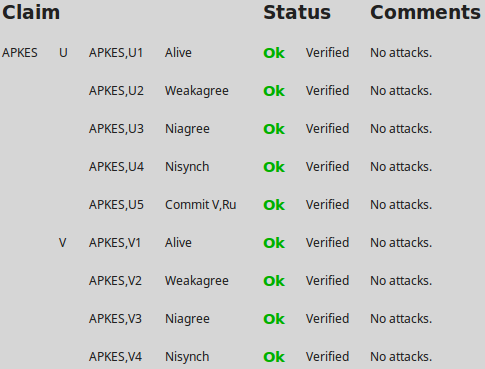
\includegraphics[scale=0.9]{Untitled.png}
	\caption{Results of a verification process using Scyther where all claims are successfully verified.}
	\label{fig:scyther-verify-claims}
\end{figure}


Scyther returns an \texttt{Ok} status code for each claim that is successfully verified. As we see in Figure \ref{fig:scyther-verify-claims}, Scyther is not able to find any attacks on the protocol. To illustrate the case of Scyther actually finding an attack, we try to verify the claims introduced in the section on secrecy, claiming that \texttt{Ru} and \texttt{Rv} are secret. In our example protocol, both nonces are sent in plaintext between U and V, hence this claim will naturally fail as seen in Figure \ref{fig:scyther-verify-claims-fail}.

\begin{figure}[h]
	\centering
	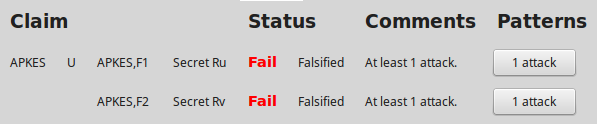
\includegraphics[scale=0.81]{ScytherFailSecretClaim.png}
	\caption{Results of a verification process using Scyther when a claim fails.}
	\label{fig:scyther-verify-claims-fail}
\end{figure}

Whenever Scyther finds an attack on a protocol, it will also provide a concrete description of the attack as graph. An example of such a graph is shown in Figure \ref{fig:scyther-graph}. It contains description of the different runs that Scyther executes, and shows how an adversary can pass messages a cross different runs to learn some secret information for constructing its attack.

\begin{figure}[h]
	\centering
	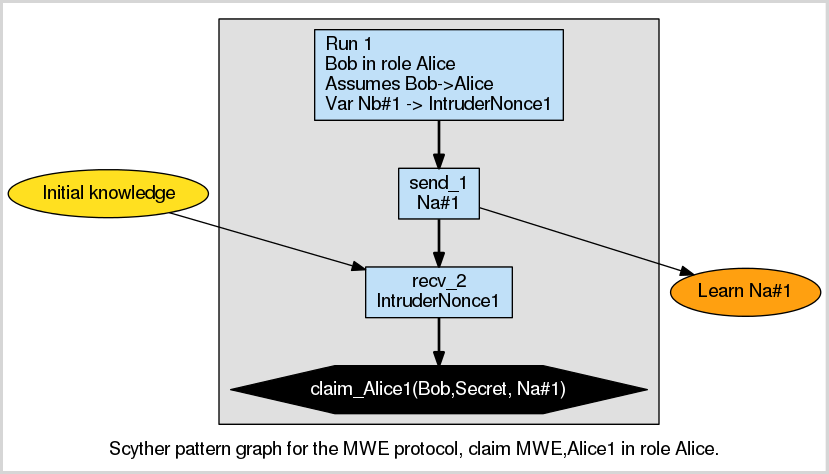
\includegraphics[scale=0.45]{ScytherFailAttackGraph.png}
	\caption{When Scyther finds an attack on a protocol, if will also provide a graph of the attack.}
	\label{fig:scyther-graph}
\end{figure}


\chapter{Three Protocols for Key Establishment in 6LoWPAN}
\label{chp:protocols}

In this chapter, three proposed protocols for key establishment in 6LoWPAN networks will be introduced. It also contains an assumption of the different security properties that would be natural to assume for the respective protocols, and a summary of the immediate weaknesses of the protocol.

\section{Adaptable Pairwise Key Establishment Scheme (APKES)}


\gls{apkes} is a proposed protocol by Krentz et al. for handling key establishment and key management in \gls{6lowpan} \cite{krentz20136lowpan}. It is currently implemented in the operating system Contiki, which is targeted at the sensor network community. As previously described, \gls{6lowpan} is a protocol stack for integrating \gls{wsn}s running on 802.15.4 with \gls{ip}v6 networks and enables the nodes in the network to communicate with each other or remote hosts over \gls{ip}. \gls{apkes} provides a framework for establishing pairwise keys for nodes in \gls{6lowpan} networks. The advantage with pairwise keys over other key schemes such as a network-shared key is related to node compromises. In \gls{6lowpan} networks, devices are often placed in potential hostile and unattended areas, significantly increasing the possibility of being tampered with by attackers.

In the case of a network shared key, the whole network would be compromised in the event of a node compromise. Also, the attacker would be able to add new nodes to the network as the upper-layer protocols rely on the 802.15.4 security sub-layer, which can filter out replayed packets and prevent injection, but not discover node compromises \cite{krentz20136lowpan}. A solution to the tampering problem could be to construct tampering-proof nodes, but this is expensive and challenging, hence not a preferable solution \cite{anderson1996tamper}. Pairwise keys, however, would only compromise the communication going to or from that particular node, and the establishment of such keys is the primary focus of \gls{apkes}.

Figure \ref{fig:6lowpan-krentz} illustrates how \gls{apkes} is implemented at the link layer along with the 820.15.4 security sublayer. In its implementation, \gls{apkes} introduces three special messages which are used in the key establishment process, namely \texttt{HELLO}, \texttt{HELLOACK}, and \texttt{ACK} \cite{krentz20136lowpan}. These are defined as 802.15.4 command messages, which are only processed by the data link layer (i.e. they are not passed to upper layers). Hence \gls{apkes} can establish pairwise keys for networks building on 802.15.4 independently from the protocols running in the upper layers.

\begin{figure}
	\centering
	\includegraphics[scale=0.80]{6lowpan-krentz.png}
	\caption{APKES is positioned in the data link layer in the 6LoWPAN stack expanding the 802.15.4 security sublayer \cite{krentz20136lowpan}.}
	\label{fig:6lowpan-krentz}
\end{figure}

\gls{apkes} provides a ``pluggable'' key establishment scheme for \gls{6lowpan} networks using pairwise keys, where the developer of a \gls{6lowpan} network picks an appropriate key establishment scheme and delegates \gls{apkes} into handling the key establishment with other nodes \cite{krentz20136lowpan}. As there is no superior scheme for \gls{6lowpan} networks, the use of pluggable schemes enhance the overall usability of the protocol, as the developer can use the most appropriate scheme based on the challenges he faces. The only function of the plugged-in scheme is to feed \gls{apkes} with the shared secret for the communicating nodes, and \gls{apkes} will handle both key establishment and key management. Examples of pluggable schemes that have been suggested for \gls{apkes} are \gls{leap} \cite{zhu2006leap+}, Blom's Scheme \cite{blom1984optimal}, and random pairwise keys \cite{chan2003random}. In the case of random pairwise keys, path key establishment has to be implemented in addition to \gls{apkes}.

During the key establishment process, a responding node goes from not being a neighbour to a tentative neighbour, before ending up as a permanent neighbour, given that the key establishment was successfully executed. The change of neighbour status is implemented to prevent \gls{dos} attacks on nodes by flooding them with messages for starting key establishments (\texttt{HELLO} messages), which would force them to reply to each message (denoted as \texttt{HELLOACK}), potentially drain their battery. Also, injecting and replaying these responses could also aid an attacker in draining the network's nodes for battery. Upon receiving a \texttt{HELLO} message, the responder ($B$) checks if the initiator ($A$) is already a neighbour, and that it has available space in its list of tentative neighbours, which is limited to $M_t$ neighbours. 

\gls{apkes} modifies the security sub-layer of 802.15.4 to discard instantly data frames that arrive from non-permanent neighbours, only accepting \texttt{HELLO}s, \texttt{HELLOACK}s, or \texttt{ACK}s. By limiting the number of tentative neighbours, $B$ is protected against consecutive \texttt{HELLO} messages, which are discarded without being processed when the number of tentative neighbours exceeds $M_t$. The list of tentative neighbours is processed for each \texttt{HELLO}, where neighbours whose expiration time has expired are deleted. The status change from a tentative to a permanent neighbour is potentially done upon receiving a valid, non-replayed \texttt{HELLOACK} or \texttt{ACK} from a non-permanent neighbour.

%\subsection{Easy Broadcast Encryption and Authentication Protocol}

%Authentication of multicast frames, however, which are sent from one node to many others and used for node discovering and network changes, are not authenticated by \gls{apkes}. Broadcast frames are authenticated with keys that are shared between neighbours, meaning that an attacker that compromises a node would not only gain access to its broadcast key, but also its neighbours' broadcast keys. As a solution for authenticating broadcast keys to achieve compromise-resilience, Krentz, Rafiee, and Meinel has suggested \gls{ebeap} to go along with \gls{apkes}. 


\subsection{Protocol specification}
\label{subsec:apkes-spec}

Key establishment in \gls{apkes} consists of a three-way handshake, as described in Figure \ref{fig:apkes-handshake}. When a node $A$ in a \gls{6lowpan} network running \gls{apkes} wants to establish contact with other nodes, it broadcasts an unauthenticated \texttt{HELLO} message containing a random nonce $Ra$. Upon receiving a \texttt{HELLO}, $B$ computes a random nonce, $Ra$, as well, and stores the concatenation of the two. $B$ then waits for a random time $T_w$. The waiting period is introduced to avoid flooding $A$ with responses, as there may be an unknown number of nodes that received the broadcasted \texttt{HELLO} message. After $T_w$, $B$ loads its key $K_{B,A}$ from the pluggable key scheme, and uses this key to authenticate a \texttt{HELLOACK} message containing the computed $R_B$ nonce and the received $R_A$. \gls{mic}s are generated by the 802.15.4 security sublayer, through the use of \gls{ccm}* operation mode in a block cipher. \gls{ccm}* is a modified version of the regular \gls{ccm} allowing for the payload of the frame to be encrypted using \gls{aes} with a 128-bit key \cite{krentz20136lowpan}. \gls{apkes} uses $K_{B,A}$ to authenticate the \texttt{HELLOACK}, and sends it to $A$. Afterwards, $B$ obtains the pairwise key $K'_{B,A}$ for future communication with $A$, by plugging $K_{B,A}$ it into the \gls{aes} algorithm along with the two nonces.

% Hvorfor sjekke at Ra er den samme? Vil ikke det være åpenbart hvis MICen ikke skulle være lik?

When $A$ receives a \texttt{HELLOACK} message, it verifies the attached \gls{mic} by extracting its key $K_{A,B}$ from the pluggable scheme and computing the \gls{mic} for the concatenation of $R_A$ and $R_B$. $A$ then computes the pairwise key for communicating with $B$ by plugging it into the \gls{aes} algorithm. $A$ also checks that the $R_A$ value has not been tampered with, and is equal to the value it initially sent in its \texttt{HELLO} broadcast. The three-way handshake ends with $A$ sending an \texttt{ACK} to $B$ that is authenticated using the pairwise key $K'_{A,B}$. When $B$ receives the \texttt{ACK}, it verifies the \gls{mic} by using its derived pairwise key $K'_{B,A}$. After this process, $A$ and $B$ have successfully agreed upon a shared pairwise key where $K'_{A,B} = K'_{B,A}$, which is to be used for encrypting all future communication between the two nodes.



%In addition to the messages \texttt{HELLO} and \texttt{HELLOACK}, the frames also contains the short addresses for the sending party. These are used

\begin{figure}[h]
\begin{tcolorbox}[title=Three-way handshake in APKES]
\begin{align*}
A:\ & Generate\ R_A\ randomly\\
A \rightarrow *:\ & \texttt{HELLO}\langle{R_A}\rangle{}\\
B:\ & Generate\ R_B\ randomly.\ Wait\ for\ T_w \leq M_w\\
B:\ & K_{B,A}\ from\ pluggable\ scheme\\
B \rightarrow A:\ & \texttt{HELLOACK}\langle{R_A, R_B}\rangle{K_{B,A}}\\
B:\ & K'_{B,A}\ =\ AES(K_{B,A}, R_A || R_B)\\
A:\ & K_{A,B}\ from\ pluggable\ scheme\\
A:\ & K'_{A,B}\ =\ AES(K_{A,B}, R_A || R_B)\\
A \rightarrow B:\ & \texttt{ACK}\langle{}\rangle{K'_{A,B}}
\end{align*}
\end{tcolorbox}
\caption{Figure of the messages sent between communicating parties during APKES' three-way handshake.}
\label{fig:apkes-handshake}
\end{figure}

\subsection{Assumptions of Security Properties}
\label{subsec:apkes-prop}

One of the focuses of \gls{apkes} is to provide authentication of parties during the key establishment process. By inspecting the messages that are exchanged between the two sides in Figure \ref{fig:apkes-handshake}, we observe that no encryption is involved in the handshake, but messages are authenticated by the use of \gls{mic}s. These \gls{mic}s are either computed using $K_{A,B}$ (the pre-shared secret) or $K'_{A,B}$ (the established pairwise key). Therefore, we can assume that entity authentication has to hold for the two communicating parties. Also, as mentioned in Section \ref{sec:attributes}, \emph{implicit} and \emph{explicit} key authentication are two of the other attributes within authentication. For a three-way handshake such as the one used by \gls{apkes}, the initiator achieves \emph{implicit} key authentication, while the responder ($B$) achieves \emph{explicit} key authentication. As the pairwise key is computed from the two nonces that are shared between $A$ and $B$, and the secret from the pluggable scheme (which we assume is secure), both know that the only parties that can compute the pairwise key are those possessing the pre-shared secret, giving them both implicit key authentication. 

$B$ also receives an \texttt{ACK} which is authenticated using the pairwise key $K'_{A,B}$, effectively meaning that $A$ has computed the pairwise key, and which $B$ can confirm by checking the attached \gls{mic}, hence it can be said to achieve explicit key authentication. From $A$'s point of view, however, it has no confirmation of that $B$ has in fact computed the pairwise key, other than it knows it has to in order to verify the authenticity of the \texttt{ACK}. Also, as \gls{apkes} is a key establishment protocol, the established key is of course claimed to be secret from the adversary.

\subsection{Weaknesses and Challenges with APKES}
\label{subsec:apkes-weakness}
% MOVE THIS TO DISCUSSION?

\gls{apkes} establishes a shared symmetric key between nodes, which is used to encrypt and decrypt data that is sent between them. One issue that the protocol does not address is the case where, for some reason, the node is forced to do a reboot. To avoid replay attacks, a node needs to keep control over the frame counters of the nodes it communicates with. These frame counters need to be swapped from the \gls{ram} memory of the device to a non-volatile storage over time. Such storages are for most 802.15.4 devices flash memory, making the swapping process both energy and time consuming \cite{krentz2015handling}. In the Contiki operating system (where \gls{apkes} is implemented), reboot commands are issued whenever processes get stuck or when replacing the battery of the device \cite{dunkels2004contiki}. In the case of a reboot without storing the frame counter, neighbouring nodes would just discard all messages from the node as the frame counter would start at zero, and the frames would be considered replayed. Another issue with storing anti-replay data is that \gls{apkes} does not remove information of disappeared neighbours (nor does it discover that a node has left the neighbourhood), which may unnecessarily seize a large part of the node's memory over time.  

In addition to the weaknesses related to frame counters and storing anti-replay protection data, \gls{apkes} has issued related to its usage of temporary and permanent neighbours. As mentioned, the life cycle of a neighbour node ranges from not being associated at all, to becoming a temporary, and finally a permanent neighbour during the key establishment process. However, \gls{apkes} discards \texttt{HELLO} messages from permanent neighbours to prevent \gls{dos} attacks. This means that if a neighbour reboots, it goes into a deadlock with former neighbours, where it is not able to establish any new keys with these nodes as its \texttt{HELLO}s would silently be discarded \cite{krentz2015handling}. The broadcasting of \texttt{HELLO}s occurs immediately after the node is booted up, which means that after the node is up and running, it will not attempt to connect to any new neighbours that may have been deployed afterwards. One can argue that it is the responsibility of the post-deployed nodes to establish contact with ``early birds'', but deployed nodes should nevertheless be able to discover new nodes during runtime. 

These issues can be applied to a real life scenario to better understand the limitations of the protocol. Assume a \gls{wsn} for medical applications with multiple devices attached to certain medical equipment. Networks around patient are not necessary stationary, as they may be moved to different facilities in the hospital. Also, certain medical equipment are very expensive, which would encourage reuse and reassignment of the devices (i.e. supporting mobility for these devices may be an important factor in certain cases). 



\section{Adaptable Key Establishment Scheme (AKES)}

The \gls{akes} aims to improve and fix the weaknesses that were introduced in \gls{apkes} and is currently implemented in the Contiki operating system \cite{krentz2015handling}. Its primary goal is to establish session keys between devices in a \gls{6lowpan} network while being able to withstand reboots and movement from one network to another. As described in Section \ref{subsec:apkes-weakness}, \gls{apkes} suffered from issues when restarting the device, and it was not able to provide any mobility. Most of these problems can be solved by one ``simple'' adjustment: Establishing session keys between nodes instead of long-term keys. By establishing session keys, \gls{mic}s from previous sessions would be invalidated, which enables the node to delete data used for providing replay protection (such as frame counters), and will also filter out old frames. Also, this removes the problem related to frame counters being reset after a reboot, as mentioned in Section \ref{subsec:apkes-weakness}. 

\gls{akes} builds on the approach from \gls{apkes}, where the underlying scheme is pluggable provides \gls{akes} with the pre-shared secret between nodes. Before an 802.15.4 node can run \gls{akes}, addressing information (which uniquely identifies a node within an 802.15.4 network and is used by the pluggable scheme when establishing the shared secret) and keying material has to be preloaded into it. \gls{akes} also has access to the same command frames \texttt{HELLO}, \texttt{HELLOACK}, and \texttt{ACK}, which are used to establish session keys, and only processed by the data link layer. Figure \ref{fig:6lowpan-krentz} describes where \gls{apkes} is implemented in the \gls{6lowpan} stack, and as \gls{akes} is merely an improvement over \gls{apkes}, it is implemented in the same layer as the 802.15.4 Security Sublayer. 

As in \gls{apkes}, \gls{akes} also utilizes a differentiation between non-neighbours, temporary neighbours, and permanent neighbours. When a node sends a \texttt{HELLO}, it obtains a temporary node status at the receiver. This status will be changed to permanent upon receipt of an authentic \texttt{ACK} message as part of the final step in the session key establishment. Keep in mind that one of the issues with \gls{apkes} was the deadlock state rebooted nodes would start in with previously permanent neighbours. In \gls{akes}, permanent neighbours who transmits a \texttt{HELLO} message will obtain a status as a temporary neighbour in addition to its old permanent neighbour status until the \texttt{ACK} is received. After receiving the \texttt{ACK}, the permanent neighbour status is deleted, and the temporary is turned into a permanent one, which effectively renews the session between the two nodes. When a permanent neighbour(i.e. a session key) is established, the neighbour is assigned an expiration time where the key becomes invalid. The lime time of a session is, however, prolonged for each received, authentic frame from the particular session, and can also be extended by issuing individual commands. 

\gls{akes} introduces two tasks for preventing deadlocks and increasing mobility for devices while still keeping \gls{dos} attacks in mind: Periodically pinging its permanent neighbours to delete disappeared nodes, and discover new neighbours by routinely broadcasting \texttt{HELLO}s. When a session with a neighbour expires, the node issues an authenticated \texttt{UPDATE} command and sends it to the node, which potentially responds with an \texttt{UPDATEACK}. A received \texttt{UPDATEACK} leads to both parties of the session extending the lifetime of their key, while the absence of such an acknowledgement, it will try a few times before eventually giving up and deleting the neighbour from its view of the network.

Trickle, which is an algorithm for distributing information in \gls{wsn}s \cite{levis2011trickle}, is adopted by \gls{akes} for discovering new neighbours in a routine matter. The challenge is to define \emph{how} often the node should broadcast \texttt{HELLO}s to discover new nodes and changes to the network topology, which Trickle aim to solve by applying different network statistics into its algorithm.

\begin{figure}[h]
\begin{tcolorbox}[title=Three-way handshake in AKES]
\begin{align*}
A:\ & Generate\ R_A\ randomly\\
A \rightarrow *:\ & \texttt{HELLO}\langle{PAN_A, ID_A, R_A, C_A}\rangle{}\\
B:\ & K_{B,A}\ from\ pluggable\ scheme\\
B:\ & Generate\ R_B\ randomly.\ Wait\ for\ T_w \leq M_w\\
B:\ & K'_{B,A}\ =\ AES(K_{B,A}, R_A || R_B)\\
B \rightarrow A:\ & \texttt{HELLOACK}\langle{PAN_A, ID_A, PAN_B, ID_B, R_B, I_{A,B}, C_B, P_A}\rangle{K_{B,A}}\\
A:\ & K_{A,B}\ from\ pluggable\ scheme\\
A:\ & K'_{A,B}\ =\ AES(K_{A,B}, R_A || R_B)\\
A \rightarrow B:\ & \texttt{ACK}\langle{PAN_B, ID_B, PAN_A, ID_A, I_{B,A}, C_A}\rangle{K'_{A,B}}
\end{align*}
\end{tcolorbox}
\caption{Figure of the messages sent between communicating parties during AKES' three-way handshake.}
\label{fig:akes-handshake}
\end{figure}

\subsection{Protocol Specification}
\label{subsec:akes-specs}

In \gls{akes}, the key establishment process consists of a three-way handshake where the two nodes establish a session key, as described in Figure \ref{fig:akes-handshake}. Initially, the node $A$ broadcasts a \texttt{HELLO} message to its neighbours containing a randomly generated nonce value $R_A$ along with the identity of the node, its \gls{pan} address, and the frame counter $C_A$. The \texttt{HELLO} broadcast is authenticated using \gls{ebeap} \cite{krentz20136lowpan}, which is a protocol for authenticating broadcast frames in \gls{6lowpan} networks, or a pre-distributed group session key.

When $B$ receives a \texttt{HELLO} transmission, generates a random nonce as well, denoted as $R_B$. It then proceeds to request the shared secret $K_{B,A}$ from its pluggable scheme, and uses this key to derive the pairwise session key $K'_{B,A}$ as $AES-128(K_{B,A}, R_A || R_B)$. $B$ then crafts a \texttt{HELLOACK} response which is sent to $A$ containing $R_B$. The \texttt{HELLOACK} is authenticated by adding a \gls{mic} generated with $K_{B,A}$, in addition to $B$'s \gls{pan} address, identity, and other values related to frame counters and \gls{ebeap} authentication.

In the response, $B$ attaches a field $P_A$ as well to indicate whether or not $A$ is currently registered as a permanent neighbour of $B$, and is also capable of piggybacking group session keys. If the $P_A$ field is set, $A$ can choose to abort the session key establishment, which would be normal if the \texttt{HELLO} was just a regular broadcast. Upon receiving the \texttt{HELLOACK}, $A$ validates the attached \gls{mic} by computing the pairwise session key $K'_{A, B}$ in the same manner as $B$. After this, future communication  is encrypted using the shared pairwise session key until it expires.


\subsection{Assumptions of Security Properties}
\label{subsec:akes-props}

\gls{akes} focuses on secure session key establishment between nodes in a \gls{6lowpan} network. As it primarily builds on \gls{apkes}, we can assume that the same security properties should hold for \gls{akes} as well. However, there are some deviations. In \gls{akes}, the responding party $B$ uses the generated session key $K'_{B,A}$ to generate the \gls{mic} that is sent in the \texttt{HELLOACK} response. By doing so, $A$ can verify that $B$ has in fact computed the session key, which can be interpreted as \emph{explicit} key authentication. Forward secrecy is often affiliated with session keys, but as the session keys are generated from a symmetric key, forward secrecy is not achievable for \gls{akes}. 



\subsection{Weaknesses}

As previously mentioned, \gls{apkes} introduced some protocol weaknesses that \gls{akes} aims to fix. While repairing most of these issues, \gls{akes} is still not perfect. For example, all addressing information (i.e. the \gls{pan} identifier, short address, and other parameters used for identifying nodes in \gls{6lowpan} networks) have to be preloaded into the node. The 802.15.4 standard has support for auto-configuring such address information at runtime, but these protocols require that the 802.15.4 security is up and running before being able to execute \cite{krentz2015handling}. \gls{akes} modifies the security sublayer of 802.15.4, which means that \gls{akes} is running before the 802.15.4 addressing protocols are running, hence they are not applicable with \gls{akes}. When \gls{akes} establishes session keys with a node, it sends the node's address and identity to the pluggable scheme in order to obtain the shared secret. This means that if \gls{akes} did not have the address of the node when it was booted up, it is not able to establish keys with it. Therefore, \gls{akes} does only support mobility for devices that are known to the node at startup.

In addition to the addressing issues, \gls{akes} is also vulnerable to attacks known has \emph{hidden wormhole attacks}. Malicious nodes may convince a node pair $A$ and $B$ that they are in fact only one hop away from each other, which is through the malicious node. This creates a ``wormhole'' between non-neighbour nodes where the attacker may disable the link to disrupt network flow, or even deny to forward certain types of frames. \gls{akes} is able to establish session keys through these wormholes, and how to mitigate them is the topic of current research \cite{krentz20146lowpan}. 

\section{Secure Authentication and Key Establishment Scheme (SAKES)}
\label{sec:sakes}

The third, and last protocol which will be discussed in this thesis is the \gls{sakes}. \gls{sakes} claims to provide secure authentication and key establishment for nodes in a device-to-device network running on \gls{6lowpan} \cite{hussen2013sakes}. Previous described protocols such as \gls{apkes} and \gls{akes} enables devices to communicate directly with each other without any previous authentication have taken place. The architecture in \gls{sakes} as seen in Figure \ref{fig:sakes-arch} consists of end devices, \gls{6lowpan} routers, \gls{6lowpan} border routers, and remote servers providing services to the devices. End devices are typically sensors, with very limited computational power. Border routers and conventional \gls{6lowpan} routers are more powerful entities which can perform lightweight public key cryptography operations.


\begin{figure}[h]
	\centering
	\includegraphics[scale=0.60]{sakes-arch.png}
	\caption{Figure of the architecture for a 6LoWPAN network using SAKES for authentication and key establishment.}
	\label{fig:sakes-arch}
\end{figure}


Border routers, also known as ``edge routers'', are in addition responsible for handling communication between the end devices and the Internet (as well as other IP-based networks), act as a broker between local data exchanged between the end devices, and generate and maintain the \gls{6lowpan} subnet \cite{olsson20146lowpan}. In \gls{sakes}, the border router is responsible for authenticating end devices and \gls{6lowpan} routers to each other, as well as generating ephemeral public-key pairs for the router to use in session key establishment. In addition to these tasks, the border router is also responsible for periodically distribute symmetric shared keys to its registered nodes.

The use of different entities with more computational power than a regular sensor device allows \gls{sakes} to provide a key establishment scheme utilizing both pairwise symmetric keys and lightweight public key cryptography. \gls{sakes} assumes that the nodes within the network are stationary are pre-registered in the border router's authentication module, which is a trusted entity between the remote server and the \gls{6lowpan} network. While not defined any where in the specification, we assume that this includes possessing the public key of the border router. 

Before a device is able to communicate with the remote server, it needs to authenticate itself to the server, as well as confirming that the nearest \gls{6lowpan} router is a authentic and valid gateway on its way to the server. The authentication module of the border router handles the authentication process, by authenticating a request sent by the end device to the router, which relays it to the edge router. This request contains the identity of the end device, the router, and the remote server. If the entities are registered in the authentication module, the border router notifies both the end device and the router with a confirmation of the other party's identity. \gls{sakes} utilizing, as mentioned, a lightweight public key approach where the border router also generates an ephemeral public key pair for the router, which is to be used for session key establishment with the remote server.

Session key establishment between the end device and remote server is done by the router acting on behalf of the end device and the server. For establishing the session key, \gls{sakes} utilizes a form of Diffie-Hellman key agreement by exchanging public keys with the remote server, before distributing the key securely to the end device.


%\gls{sakes} was suggested as a scheme for securing communication for device-to-device communication 


\subsection{Protocol Specification}
\label{subsec:sakes-spec}

\gls{sakes} consists of two phases: Authentication and session key establishment. Figure \ref{fig:sakes-auth} describes the messages exchanged between the end device ($A$), the \gls{6lowpan} router ($B$), and the border router ($C$) in the authentication phase of \gls{sakes}. $A$ starts the authentication by generating a random nonce $N_A$, which it transmits to its closest router $B$. The router responds by generating its own random nonce $N_B$, and sends this back to $A$. The identities of the end device, the nearest router of the end device, and the remote server the device wants to connect to is then encrypted into the ciphertext $C_A$ by $A$ using the symmetric key $K_{AC}$, which is shared between the end device and the border router. $A$ also then sends this ciphertext along with its identity and previously computed nonce to the router after adding a \gls{mac-auth} of the message using the shared key $K_{AB}$.

Upon receiving the request from $A$, $B$ authenticates the \gls{mac-auth} of the message by using its copy of the secret key $K_{AB}$, and adds its nonce $N_B$ to the message. The request is authenticated by $B$, who generates a \gls{mac-auth} using $K_{BC}$ and relays it to the border router $C$. When the request is received by $C$, it verifies the attached \gls{mac-auth} by using its copy of the symmetric key that it shares with $B$. It then decrypts the ciphertext created by $A$ containing the identity of the end device, the router, and the remote server by using the symmetric key $K_{AC}$.


\begin{figure}[h]
\begin{tcolorbox}[title=Authentication in SAKES]
\begin{align*}
A:\ & Generate\ N_A\ randomly\\
A \rightarrow B:\ & N_A\\
B:\ & Generate\ N_B\ randomly\\
B \rightarrow A:\ & N_B\\
A:\ & Construct\ C_{A}:\ \{ID_A, ID_B, ID_D\}_{K_{AC}}\\
A \rightarrow B:\ & \langle{C_A, ID_A, N_A}\rangle{K_{AB}}\\
B \rightarrow C:\ & \langle{C_A, ID_B, N_B}\rangle{K_{BC}}\\
C:\ & Verify\ the\ identity\ of\ A,\ B,\ and\ D\\
C: \ & Construct\ S_C: \{ID_A, ID_B, ID_D\}_{Sk_{C}}\\
C:\ & Generate\ N_C\ randomly\ and\ a\ public\ key\ pair\ (Pk_B, Sk_B)\\
C \rightarrow B:\ & \{N_C, S_C, Pk_B, Sk_B\}_{K_{BC}}\\
C \rightarrow A:\ & \langle{ID_B, N_C}\rangle{K_{AC}}\\
\end{align*}
\end{tcolorbox}
\caption{Figure of the messages sent between the end device (A), router (B), and border router (with authentication module) (C) in SAKES' authentication phase.}
\label{fig:sakes-auth}
\end{figure}

The border router then checks with its authentication module whether the message is sent by the end device $A$, and if the identity of its nearest neighbour router $B$ is correct. If these checks are successful, the border router creates a signed message $S_C$ containing the identities of the end device, router, and remote server. It also generates a public key pair $(Pk_B, Sk_B)$ based on \gls{ecc}, and random nonce $N_D$. It then sends two messages: one to the router, and one to the end device. The message sent to $B$ contains the nonce $N_D$, the signed message $S_C$ containing the verified identities of the request, and the public key pair for $B$ to use in the key establishment phase. To provide secrecy for the generated key pair, the entire message is encrypted under the shared symmetric key $K_BC$ to ensure that the key pair is only accessible to $B$. The end device $A$ also receives a confirmation message from $C$ containing the identity of the router, as well as the random nonce $N_D$ to prevent replaying. The message is authenticated using a \gls{mac-auth} with the shared secret $K_{AC}$ as the key to ensure its authenticity.

After both the end device and the router receives their confirmation messages and successfully verifies their authenticity, the authentication process is believed to be completed. The next step in \gls{sakes} is for the router $B$ to establish a session key with the remote server $D$ on behalf of the end device $A$, as the end device often has limited computational power. The messages sent between the entities in the key establishment phase of \gls{sakes} can be seen in Figure \ref{fig:sakes-keys}.

\begin{figure}[h]
\begin{tcolorbox}[title=Key Establishment in SAKES]
\begin{align*}
B \rightarrow D:\ & \{C_C, N_B, Pk_B, B, hash\}_{Sk_B} \\
D:\ & Calculate\ Session\ Key\ (SK_D):\ SK_D = g^{Pk_B * Sk_D} \mod{P}\\
D:\ & Generate\ N_D\ randomly\\
D \rightarrow B:\ & \{Pk_D, P, g, N_D, hash\}_{Sk_D}\\
B:\ & Calculate\ Session\ Key\ for\ A\ (SK_A):\ SK_A = g^{Pk_D * Sk_B} \mod{P}\\
B \rightarrow A:\ & \{SK_A, N_B\}_{K_{AB}}\\
Claim:\ & SK_A = SK_D\\
\end{align*}
\end{tcolorbox}
\caption{Figure of the messages sent between communicating parties in SAKES' key establishment between the end device (A), the 6LoWPAN router (B), and the remote server (D).}
\label{fig:sakes-keys}
\end{figure}

The router crafts a request containing the obtained signed proof from the border router, its identity, and the random nonce $N_B$, and it also adds its temporary public key $Pk_B$. Also, $B$ computes a hash of the message and appends it as well, before signing it. By signing the message using its corresponding private key $Sk_B$, $B$ allows the remote server to verify the authenticity of the message by using the attached public key $Pk_B$. The server then checks the authenticity of the signed proof in the message that the authentication module in $C$ created by applying its copy of $C$'s public key.

The computation of the session key $SK_D$ in \gls{sakes} is displayed in Equation \ref{eq:skd}, allegedly utilizing a version of the Diffie-Hellman key agreement. In the equation, $g$ and $P$ are two cryptographic numbers, respectively a generator and a prime modulus, while the exponents are the public key of the router $B$ and the private key of the server $D$. After generating the session key, $D$ constructs a message to $B$ containing its public key, a random nonce $N_D$, and the two cryptographic numbers $g$ and $P$. A hash of the message is attached as well, before it is signed using the remote server's private key $Sk_D$, and sent to $B$. 

\begin{equation}
\label{eq:skd}
SK_D = g^{\ Pk_{B}\ *\ Sk_D} \mod P
\end{equation}

Upon receiving the response from the remote server, $B$ computes the hash for the message and compares it to the attached hash value, as well as verifying that the signature matches the public key. The session key for the end device is computed as in Equation \ref{eq:ska}, using the received cryptographic numbers $g$ and $P$, and the public key of $D$ and $B$'s ephemeral private key. In order to distribute the session key securely to the end device $A$, the key is encrypted along with the nonce $N_B$ under the symmetric key $K_{AB}$, and sent to $A$. After the end device successfully decrypts and retrieves its session key, future communication between $A$ and $D$ will be encrypted using the session key. 

\begin{equation}
\label{eq:ska}
SK_A = g^{\ Pk_{D}\ *\ Sk_B} \mod P
\end{equation}


\subsection{Assumptions of Security Properties}
\label{subsec:sakes-props}

\gls{sakes} uses an authentication module located in the border router to authenticate end devices and routers before granting them a signed proof to use in the key establishment process. Authentication is one of the most fundamental security properties in a key establishment, and therefore it is fair to assume that \gls{sakes} should provide authentication between end devices, routers, and border routers. The key establishment process is merely conducted between the router and the remote server, where the remote server has no knowledge of the end device while the border router is absent from this phase. Therefore, we assume that authentication in this process is claimed between the end device and the router, and between the router and the remote server.

As \gls{sakes} makes use of both pairwise keys and public key pairs, the generated session keys should, of course, be claimed to be secret. Also, the private key of the ephemeral key pair generated the authentication module should be secret to ensure the secrecy of the generated session key. In modern key establishment schemes, the Diffie-Hellman key agreement process can be used to provide forward secrecy for communicating parties. In \gls{sakes}, the remote server holds a long-term public key pair, while the border router generates a fresh ephemeral key pair for each session. Nevertheless, forward secrecy should be a desirable property for protocols that leverage Diffie-Hellmen. 


\subsection{Weaknesses}

The major downside with \gls{sakes} is that the authors have misunderstood the concept of Diffie-Hellman key agreement. If we look closer at the two equations that derive the alleged identical session keys, we observe that they are in fact unequal. The mathematical equation for Diffie-Hellman is listed in Equation \ref{eq:dh} below.

\begin{equation}
\label{eq:dh}
(g^a \mod p)^b \mod p = (g^b \mod p)^a \mod p
\end{equation}

In \gls{sakes}, the private key of the remote server and the ephemeral public key of the router are used to calculate the session key at the server's side. However, the router uses its ephemeral private key and the public key of the server to compute the session key, which gives us two different session keys as shown in Equation \ref{eq:dh-wrong}.

\begin{equation}
\label{eq:dh-wrong}
(g^a \mod p)^b \mod p \neq (g^c \mod p)^d \mod p
\end{equation}

As for the computation of the key, the remote server has a fixed public key pair which is used for generating every session key, while the router uses a freshly generated key pair that it gets from the border router. The Diffie-Hellman key agreement relies on the mathematical challenge in computing discrete logarithms (i.e. finding $x$ when presented with $g^x$), and having half the key fixed for each session key can potentially leak information about the secret key over time.

Also, the authors seem to have misused the notation of \gls{mac-auth} in the key establishment phase, where they generate \gls{mac-auth}s using publicly known keys such as $Pk_B$ and $Pk_D$ instead for a shared secret key, which is the conventional way of applying such functions. Lastly, the protocol specifications uses private keys to sign the messages that are exchanged during the key establishment, but the public keys that should be used to verify the signed messages are not published at any secure server. Also, the public key that should be used to verify the signature is sent within the signed message, which can remind of a self-signed certificate. While the identities of the end device and the router are verified through the signed message $C_C$ created by the authentication module, it does not verify that the public key pair used for the key establishment is the same that was generated by the border router.



\chapter{Formal Security Analysis of Three Key Establishment Protocols}
\label{chp:analysis}


\section{Modelling Security Properties}

As mentioned in Section \ref{sec:attributes}, key establishment schemes desire certain security properties. In the verification of the security protocols of this thesis, the following properties are verified: \emph{Entity authentication}, \emph{Implicit key authentication}, \emph{Explicit key authentication}, \emph{Known-key secrecy}, \emph{Key control}, and \emph{Secrecy of key}. As mentioned in Section \ref{sec:attributes}, symmetric key establishment schemes are not resilient against \gls{kci} attacks, and do not provide forward secrecy. These properties are nevertheless included in the models as \gls{sakes} uses a lightweight version of public-key cryptography and the type of Diffie-Hellman key agreement to establish session keys.

\paragraph{Entity authentication} Entity authentication between nodes corresponds to the security claim \texttt{Alive}, and can also be verified through stronger claims such as \texttt{Weakagree}. This property can only be violated if the adversary is able to inject or tamper with messages that are transmitted over the network, which we assume that the adversary in a \gls{6lowpan} network is.

\paragraph{Implicit key authentication} Implicit key authentication is modelled through the settings of the adversary compromise model described in Section \ref{sec:adversary}. The property is modelled by allowing the adversary to obtain the long-term keys and impersonate anyone except for the nodes that are supposedly establishing keys.

\paragraph{Explicit key authentication} Is achieved when the protocol satisfied both implicit key authentication and key confirmation. This is modelled through the security claim for non-injective agreement denoted as \texttt{ni-agree}, but can also be modelled by using \texttt{running} and \texttt{commit} claims.

\paragraph{Known-key security} By revealing session keys to the adversary after usage (i.e. the session key is expired, and will never be used again) known-key security can be modelled. This is done by setting the \emph{Session-key reveal} rule in the adversary compromise model.

\paragraph{Key control} Scyther has no support for verifying key control. Therefore, this security property has to be verified by hand. 

\paragraph{Secrecy of key} To model a key (or any other property) as secret, the \texttt{secrecy} claim is used in Scyther.

\paragraph{Forward secrecy} Both \gls{pfs} and \gls{wpfs} are related to active adversaries, and is modelled through the adversary compromise model, which can be configured to leak the long-term private key which the session keys are derived from.

\paragraph{Key compromise impersonation} \gls{kci} is also a property related to an active adversary, and is therefore available through the adversary model where the adversary can be allowed to obtain the long-term private key of the actors.


\section{Formal Security Analysis of APKES}
\label{sec:apkes-analysis}

\gls{apkes} is modelled as two roles, the initiator $A$ and the responder $B$, agreeing upon a pairwise key through the message exchange that is presented in Figure \ref{fig:apkes-handshake}. There is not specified any concrete type of pluggable scheme (i.e. the scheme where \gls{apkes} obtains the shared secret between two nodes), hence we assume that whatever scheme is used is secure. In the model, the shared secret obtained from the pluggable scheme has been modelled using Scyther's built-in support for shared symmetric keys, where the two nodes $A$ and $B$ both possesses the shared secret at start-up.

\gls{apkes} states that the $R_A$ value has to be checked whether or not it has been tampered with, before the pairwise key can be derived at the initiating side. This can be verified by modelling the protocol to agree upon the $R_A$ value during the protocol execution, and committing to this. In addition, we model agreement over the pairwise key by using a \texttt{Running} claim in role $B$ after receiving the \texttt{ACK} authenticated with the pairwise key, and \texttt{Commit} claims in both roles to claim explicit key authentication on the pairwise key. As $B$ authenticates the $HELLOACK$ by using the shared secret, we do not claim that the pairwise key is created before $A$ receives the $HELLOACK$ from B. The Scyther model of \gls{apkes} can be viewed in its entirety in Appendix \ref{app:apkes}.

\subsection{Security Claims}

By taking starting point in the protocol specification from Section \ref{subsec:apkes-spec} and the alleged security properties from Section \ref{subsec:apkes-prop}, the protocol is modelled as an \gls{spdl}-script, which can be verified by Scyther. Listing \ref{lst:claims-a-apkes} describes the various security claims that is chosen for $A$. In these claims, we verify that the other party in the protocol is authentic, and that the pairwise key is secret. Claims for non-injective synchronization and agreement is also added to verify that the protocol executes as expected. The security claims for role $B$ in \gls{apkes} are stated in Listing \ref{lst:claims-b-apkes}. Compared to the claims for $A$, $B$ does not contain the \texttt{Commit} claim for the variable $N_A$, as the \texttt{Running}, \texttt{Commit} approach is used in role $A$ to provide agreement (i.e. confirm that the nonce has not been altered by $B$) over the nonce $N_A$. We also claim non-injective synchronization and agreement.\\

\begin{lstlisting}[caption={Security claims for role A in APKES.}, label={lst:claims-a-apkes}]
	claim(A, Alive);
	claim(A, Weakagree);
	claim(A, Niagree);
	claim(A, Nisynch);
	claim(A, Commit, B, Na);
	claim(A, Secret, PairwiseKey);
	claim(A, Commit, B, PairwiseKey);
\end{lstlisting}


\begin{lstlisting}[caption={Security claims for role B in APKES.}, label={lst:claims-b-apkes}]
	claim(B, Alive);
	claim(B, Weakagree);
	claim(B, Niagree);
	claim(B, Nisynch);
	claim(B, Secret, PairwiseKey);
	claim(B, Commit, A, PairwiseKey);
\end{lstlisting}


\subsection{Adversary}

In the description of \gls{apkes}, no specific adversary is mentioned. We assume that such a protocol would be used for key establishment in \gls{6lowpan} networks, which are potentially deployed in hostile areas. Therefore, we can assume that the adversary would be able to observe, inject, and tamper with messages that are sent over the network. As \gls{apkes} does not utilize any session keys, but rather agreeing upon a fixed long-term key, we model the adversary in a Dolev-Yao way without giving it any active capabilities other than being able to obtain the long-term keys of nodes not participating in the current key establishment process. 

\subsection{Results}

Figure \ref{fig:apkes-verified} shows the verification result from running the model of \gls{apkes} through Scyther in the presence of the adversary described above. Scyther was able to perform an unbounded verification of the model where all claims but one were successfully verified. \gls{apkes} provides verifiable entity authentication, explicit key authentication for role $B$ (implicit for $A$), and holds the non-injective synchronization property, which means that every message in protocol is executed as expected, even in the presence of the adversary. When looking at the characterization of the protocol, there exist only one executable trace for each of the roles. Hence, there does not exist any malicious behaviour that can force the modelled protocol to misbehave. The attack proposed by Scyther on $Commit\ B, \{Na, Nb\}k(A,B)$ is not a direct attack on the protocol, but it shows that it is not possible to achieve explicit key authentication for the role $A$, as it has no knowledge of if $B$ has computed the pairwise key. 


\begin{figure}[h]
	\centering
	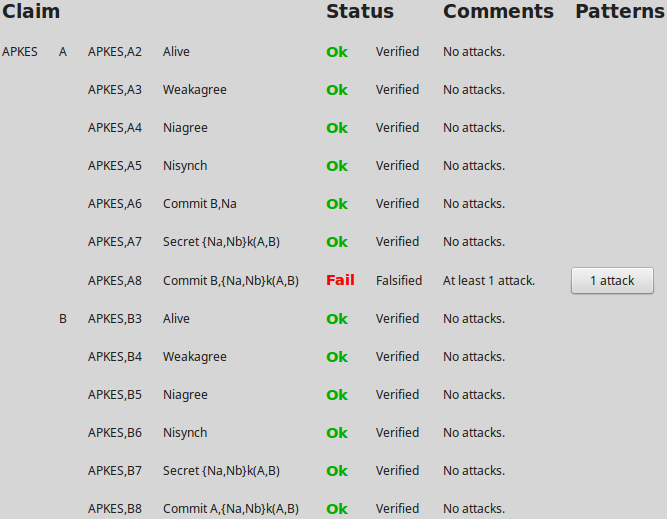
\includegraphics[scale=0.75]{analysis/apkes-verified.png}
	\caption{Result of verifying APKES' security claims using Scyther.}
	\label{fig:apkes-verified}
\end{figure}



\section{Formal Security Analysis of AKES}
\label{sec:akes-analysis}

\gls{akes} is modelled almost as its predecessor, but with additional content that is used to allow mobility for the devices. As \gls{akes} is used for establishing session keys, the \texttt{SKR} claim is used emphasize that the key is in fact a session key. The pluggable scheme is assumed to be secure, and is modelled as a symmetric key shared between the two communicating parties using Scyther's built-in symmetric key support. Appendix \ref{app:akes} contains the model in its entirety. \gls{apkes} was not able to provide explicit key authentication of role $B$ for the initiator $A$. In \gls{akes}, however, the received \texttt{HELLOACK} is authenticated using the session key. Therefore, we model a \texttt{Running} claim (not present in Listing \ref{lst:claims-a-akes} or \ref{lst:claims-b-akes} - See Appendix \ref{app:akes}) to indicate that the role $B$ has computed the key at this point in time and a \texttt{Commit} claim to state that the two parties agree that the session key has been computed.

\subsection{Security Claims}

From the protocol specification in Section \ref{subsec:akes-specs} and the assumed security properties in Section \ref{subsec:akes-props}, the security claims that are claimed to hold for the two roles in \gls{akes} are listed in Listing \ref{lst:claims-a-akes} and Listing \ref{lst:claims-b-akes}. In addition to claiming authentication for the other party, we also claim that the protocol has been executed as intended by adding claims for non-injective synchronization and agreement.\\

\begin{lstlisting}[caption={Security claims for role A in AKES.}, label={lst:claims-a-akes}]
	claim(A, SKR, SessionKey);
	claim(A, Alive);
	claim(A, Weakagree);
	claim(A, Niagree);
	claim(A, Nisynch);
	claim(A, Commit, B, SessionKey);
\end{lstlisting}


\begin{lstlisting}[caption={Security claims for role B in AKES.}, label={lst:claims-b-akes}]
	claim(B, SKR, SessionKey);
	claim(B, Alive);
	claim(B, Weakagree);
	claim(B, Niagree);
	claim(B, Nisynch);
	claim(B, Commit, A, SessionKey);
\end{lstlisting}

\subsection{Adversary}

The adversary in this model is nearly the same adversary as the one introduced in the verification of \gls{apkes}. However, in order to model session keys, the adversary is allowed to obtain all session keys whose identifier differs from the current protocol execution. 

\subsection{Results}

Figure \ref{fig:akes-verified} shows the result of running the model of \gls{akes} through Scyther in the presence of the adversary presented above, where \gls{akes} is verified for an unbounded state space and all the claimed security properties are successfully verified. \gls{akes} provides provable authentication for both roles, as well as explicit key authentication. In addition, \gls{akes} is proved to hold the non-injective synchronization and data agreement claims which state that the protocol was executed as intended. When looking at the characterization of \gls{akes} only one possible trace is returned for each role, which means that there exists only one way to execute the protocol.

\begin{figure}[h]
	\centering
	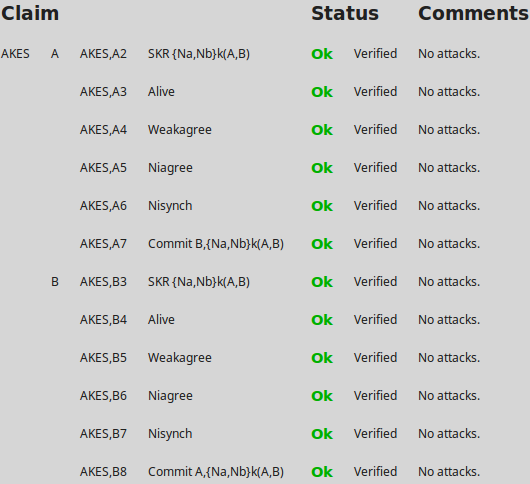
\includegraphics[scale=0.95]{analysis/akes-verified.png}
	\caption{Result of verifying AKES' security claims using Scyther.}
	\label{fig:akes-verified}
\end{figure}


\section{Formal Security Analysis of SAKES}
\label{sec:sakes-analysis}

From the protocol specification in Section \ref{subsec:sakes-spec} and the assumed security properties in Section \ref{subsec:sakes-props}, \gls{sakes} have been modelled into four roles: $A$ (End device), $B$ (Router), $C$ (Border router), and $D$ (Server). The authentication phase is carried out between $A$, $B$, and $C$, before $B$ and $D$ establish the session key, which is distributed from the router $B$ to the end device $A$. As the protocol specification presented in the original protocol proposal can be considered inconsistent, some assumptions have been made in the model.

The verification of the original protocol in its entirety takes over 72 hours to complete on a workstation with an Intel Core i7 processor with four cores and 12 GB \gls{ram} (The experiment was aborted at this point). Therefore, it has been infeasible to formally verify the complete protocol in one round, hence the two phases have been separated into different models to be able to provide some insight on the weaknesses of \gls{sakes}. The two models are available in Appendix \ref{app:sakes-auth} and \ref{app:sakes-keys}. There may, however, be additional attacks on the protocol that the analysis of these models is unable to detect. Especially as the nonces $N_A$, $N_B$, and $N_C$ are re-used in the key establishment phase, but the models are unable to link these values between protocols, the usage of these nonces in the key establishment phase may lead to attacks as they are freshly generated.


\subsection{Authentication Phase}
\label{subsec:sakes-auth}

\subsubsection{Security Claims}

The end device $A$ is only in direct communication with the router $B$ and the border router $C$, which is why authentication is only claimed for these two roles as seen in Listing \ref{lst:claims-a-sakes-auth}. We add claims for non-injective synchronization and agreement to find attacks where the messages are not exchanged as intended.\\

\begin{lstlisting}[caption={Security claims for role A during the authentication phase in SAKES.}, label={lst:claims-a-sakes-auth}]
	claim(A, Alive, B);
	claim(A, Alive, C);
	claim(A, Weakagree, B);
	claim(A, Weakagree, C);
	claim(A, Niagree);
	claim(A, Nisynch);
\end{lstlisting}


Listing \ref{lst:claims-b-sakes-auth} contains the claims that are stated for role $B$ (i.e. the \gls{6lowpan} router) in \gls{sakes} during the authentication phase. The router is originally interacting with all the other entities in the network, but during the authentication it only interacts with the end device $A$, and the border router $C$. Hence we are claiming authentication for only these roles. In addition, we state that the ephemeral key $Sk_B$, which is generated by the border router during the authentication phase and which is to be used in the key establishment, is secret. To verify that the role behaves as intended, we add claims for non-injective synchronization and agreement.\\

\begin{lstlisting}[caption={Security claims for role B during the authentication phase in SAKES.}, label={lst:claims-b-sakes-auth}]
	claim(B, Secret, Sk);
	claim(B, Alive, A);
	claim(B, Alive, C);
	claim(B, Weakagree, A);
	claim(B, Weakagree, C);
	claim(B, Niagree);
	claim(B, Nisynch);
\end{lstlisting}

The border router $C$ does only participate in the authentication phase with $A$ and $B$, hence we claim authentication for these two parties. In addition we add claims for non-injective synchronization and agreement to state that the protocol was executed as expected as seen in Listing \ref{lst:claims-c-sakes-auth}.\\

\begin{lstlisting}[caption={Security claims for role C during key establishment in SAKES.}, label={lst:claims-c-sakes-auth}]
	claim(C, Alive, A);
	claim(C, Alive, B);
	claim(C, Weakagree, A);
	claim(C, Weakagree, B);
	claim(C, Niagree);
	claim(C, Nisynch);
\end{lstlisting}

\subsubsection{Adversary}

For the authentication phase in \gls{sakes} we assume a Dolev-Yao adversary which is capable of eavesdropping, delete messages, compute cryptographic analysis on intercepted messages, forge new messages from its knowledge, and insert them into the network. 

\subsubsection{Results}

Figure \ref{fig:sakes-verified-auth} shows the result of verifying \gls{sakes}' authentication phase, where multiple of the claimed security properties are falsified. Scyther is able to verify that \gls{sakes} provides entity authentication for the end device, router, and border router, but fails to provide stronger notions of authentication such as weak agreement for the end device. Also, the authentication phase in \gls{sakes} does not provide non-injective synchronization nor non-injective data agreement for either of the three roles. The attacks presented below are described more thoroughly in Section \ref{subsec:sakes-fix}, and improvements are suggested to achieve the claimed security properties.

\begin{list}{•}{}

\item \texttt{SAKES\_AUTH, A3 \& A4 Weakagree B \& C}: The attacks proposed by Scyther that falsifies the \texttt{weakagree} claims for the end device leverage the last message that is sent between the end device and the border router, and can be seen in Appendix \ref{fig:sakes-attack-weakagree}. When the border router receives the relayed request from router, it has to confirm the identity of the router to the end device. There are, however, flaws in the messages that are exchanged, which enables an adversary to use the request created by the end device and the nonce generated by the router to change a different end device's perception of its closest router.

\item \texttt{SAKES\_AUTH, A6 \& B7 \& C6 Nisynch}: Neither $A$, $B$, or $C$ is able to hold the non-injective synchronization property. If we study the attack proposed in Appendix \ref{fig:sakes-attack-nisynch}, we see that the adversary is using the same approach as in the attack on the \texttt{weakagree} above. In the original protocol description of \gls{sakes}, the adversary is able to combine the information sent in the second and third message into a message that is sent directly to the border router. Such an alternation is the message flow is not allowed in the model of the protocol, and hence the \texttt{nisynch} properties are falsified.

\item \texttt{SAKES\_AUTH, A6 \& B7 \& C6 Niagree}: Scyther also proposes attacks targeting the non-injective agreement claims. These attacks are of the same flavour as the attacks targeted at the \texttt{nisynch} property above, and the claims are falsified as the adversary is able to combine information in observed messages into valid new messages. Generation of new messages lead to a different set of data items, hence the protocol is not able to agree upon the data that is exchanged throughout the protocol.

\end{list}

\begin{figure}[h]
	\centering
	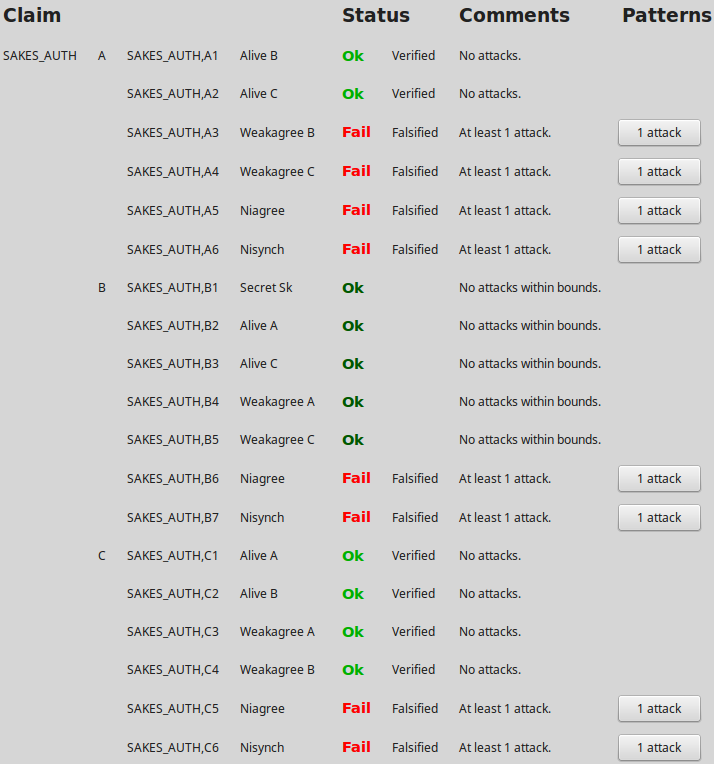
\includegraphics[scale=0.68]{analysis/sakes-auth-verified.png}
	\caption{Result of verifying SAKES' authentication claims using Scyther.}
	\label{fig:sakes-verified-auth}
\end{figure}

\newpage

\subsection{Key Establishment Phase}

In order to model the key establishment phase in \gls{sakes}, it is assumed that the Diffie-Hellman key agreement is done correctly by letting $B$ and $D$ share their secret key to the power of the generator $g$. In addition, it is assumed that when the authors use notion of ``decrypting the ciphertext encrypted with the private key of $X$'', they actually mean that the message is signed using the private key of $X$, and that the signature can be verified by applying the corresponding public key. When it comes to the notation of \gls{mac-auth}s, an assumption is that the alleged \gls{mac-auth} that is sent between the router and the server that do not share any symmetric key is simply a hash of the message.

Originally, the server distributes the generator $g$ and the prime modulus $P$ to the router. This means that a new message needs to be introduces to allow for the Diffie-Hellman procedure to be executed correctly. If the router $B$ either has the these two cryptographic numbers preloaded in its memory, or if they get distributed from the border server, the router is able to send $g^{Sk_B}$ to the server in its first message. As the original protocol specification got the Diffie-Hellman part wrong, the models presented in this section assume that the router has access to both $g$ and $P$ before initiating the key establishment process with the remote server $D$.


\subsubsection{Security Claims}

The session key establishment in \gls{sakes} is conducted between the router $B$ and the server $D$, before the session key is distributed from the router to the end device $A$. We assume that $A$ and $B$ have authenticated each other before the key establishment process is engaged. Listing \ref{lst:claims-a-sakes-key} shows the claims that is stated for the end device in the key establishment phase of \gls{sakes}. Since the only message that is sent between the two contains the session key, which is encrypted with their shared symmetric key $K_{A,B}$, we assume that the session key is secret by using the \gls{skr} claim. In addition, claims for non-injective synchronization and agreement have been added to ensure that the protocol is executing as expected based on the model.\\

\begin{lstlisting}[caption={Security claims for role A during key establishment in SAKES.}, label={lst:claims-a-sakes-key}]
	claim(A, Niagree);
	claim(A, Nisynch);
	claim(A, SKR, SessionKeyA);
\end{lstlisting}

As the router generates the session key on behalf of the end device $B$, we also state that the session key should be secret at the router side using the \gls{skr} claim as seen in Listing \ref{lst:claims-b-sakes-key}. As the router interacts with the remote server $D$, we also add claims for entity authentication. Finally, claims for non-injective synchronization and data agreement are added to verify that the protocols behaves as specified in the protocol model. \\

\begin{lstlisting}[caption={Security claims for role B during key establishment in SAKES.}, label={lst:claims-b-sakes-key}]
	claim(B, Alive, D);
	claim(B, Weakagree, D);
	claim(B, Niagree);
	claim(B, Nisynch);
	claim(B, SKR, SessionKeyA);
\end{lstlisting}


For the remote server, authentication is claimed only between it and the router which is establishes session keys with. The end device is indirectly authenticated through the proof that is signed by the authentication module in the border router, but this is not modelled as a direct authentication claim in this model. The generated session key $SessionKeyD$ is claimed to be secret using the \texttt{SKR} notation. In addition, we also claim non-injective synchronization and agreement for the role as seen in Listing \ref{lst:claims-d-sakes-key}.\\


% run verification with Alive, Weakagree, for A?
\begin{lstlisting}[caption={Security claims for role D during key establishment in SAKES.}, label={lst:claims-d-sakes-key}]
	claim(D, Alive, B);
	claim(D, Weakagree, B);
	claim(D, Niagree);
	claim(D, Nisynch);
	claim(D, SKR, SessionKeyD);
\end{lstlisting}

\subsubsection{Adversary}

For the key establishment phase, we assume a Dolev-Yao adversary which is capable of eavesdropping, delete messages, compute cryptographic analysis on intercepted messages, forge new messages from its knowledge, and insert them into the network. It is allowed for the adversary to obtain the session keys for all sessions whose identifier differs from the current session's identity. As \gls{sakes} utilizes a form of Diffie-Hellman key agreement, it is also assumed that the protocol should possess forward secrecy, especially since the half of the key is fixed as the remote server uses a permanent public key pair.

\subsection{Results}

The results of verifying the model of the key establishment phase in \gls{sakes} using Scyther is presented in Figure \ref{fig:sakes-verified-keys}. Entity authentication of both the router and the server is provided and verified in the key establishment process, but stronger notion such as \texttt{Weakagree} for the server $D$ is falsified for the router $B$ in this model. Both non-injective synchronization and data agreement are falsified for each of the roles in the key establishment phase. \gls{sakes} achieves known-key secrecy of the computed session key for both the router and the server, as well as the end device who receives the session key from the router.  If the model is run in presence of an adversary that is allowed to obtain the long-term private key, the generated session key is falsified, as \gls{sakes} does not provide forward secrecy.

\begin{figure}[h]
	\centering
	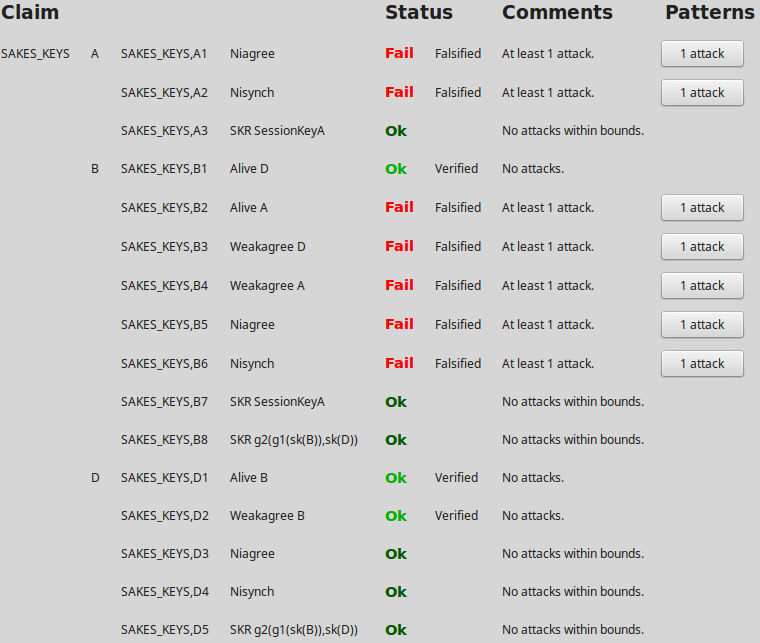
\includegraphics[scale=0.65]{analysis/sakes-keys-verified.png}
	\caption{Result of verifying SAKES' key establishment claims using Scyther.}
	\label{fig:sakes-verified-keys}
\end{figure}

\begin{list}{•}{}

\item \texttt{SAKES\_KEYS, A2 \& B4 \& D4 Nisynch}: The attacks on the non-injective synchronization claim are shown in Figure \#. In this attack, the adversary extracts the proof from the intercepted message, and generates its own public key pair and nonces in order to 	forge a message to the remote server. However, as the server verifies the identities within the the proof it is questionable whether this attack manifests in a full-size model of the protocol which includes both phases.

\item \texttt{SAKES\_KEYS, A1 \& B3 \& D3 Niagree}:

\item \texttt{SAKES\_KEYS, B2 Weakagree D}: Because the proof is not returned.
\end{list}


\section{Limitations in the Analysis}

Even though Scyther is a powerful tool for formal security analysis, there are certain types of attacks that it is not able to model. Replay attacks, where the adversary saves a captured frame for injecting it into the network at a later time, are not possible to model in Scyther. Both \gls{akes} and \gls{apkes} claim to avoid replay attacks through the 802.15.4 security sub-layer and the use of frame counters to discover frames that have been previously observed \cite{krentz2015handling, krentz20136lowpan}.

\gls{sakes} claims to prevent replay attacks by adding nonces and \gls{mac-auth}s to prevent messages from being tampered with and to ensure freshness \cite{hussen2013sakes}. This analysis does not, however, verify these claims. As the \gls{sakes} protocol proved to be computational expensive to verify on the available equipment, it has been divided into two separate protocols. While the analysis finds certain attacks on the two phases, there may be additional attacks that the models are unable to detect.

The big weakness with this analysis is that the mutual authentication that is achieved between $A$, $B$, and $C$ in the authentication phase is not transferable to the key establishment phase. Therefore, the necessary values are freshly generated at the appropriate places. For example are the nonce $N_C$ generated at the router $B$ before the router sends its first message in the key establishment phase.  


% Litt mer?

%For example could an adversary be able to establish the session key with a different entity than what was originally intended.



% How to check for properties:

% Forward Secrecy: Not able to achieve in symmetric key. Check through Scyther rules.

% Known-Key Security: Session-Key reveal

% Key Confirmation: running, commit / niagree

% Key Compromise Impersonation: Impossible to achieve in protocols relying on symmetric keys? Need asymmetric? Boyd book. SKR claim of an entity whose long-term key is revealed to the adversary

% Unknown key share: Known-Key Security?

% Entity authentication: From A to B: Aliveness of A in B's claims.

% Implicit: Long-term reveal for other entities than A and B.

% Explicit. Implicit + key confirmation




%As \gls{sakes} uses Diffie-Hellman, which Scyther does not originally support, a ``hack'' has been introduced to enable Scyther to interpret $(g^a)^b$ and $(g^b)^a$ as equal. Diffie-Hellman can be modelled by introducing a helper protocol in Scyther that underapproximates $g^{x}$ into $hashfunction(g, x)$. The helper protocol is shown in Listing \ref{lst:helper} and is marked with the at-symbol (@). This allows Scyther to interpret the two terms $g2(g1(T1),T2)$ and $g2(g1(T2), T1)$ as approximate equal \cite{scyther-manual}.\\
%
%\begin{lstlisting}[caption={Helper protocol to model Diffie-Hellman in SAKES.}, label={lst:helper}]
%hashfunction g1, g2;
%
%protocol @exponentiation(DH)
%{
%	role DH
%	{
%		var T1,T2: Ticket;
%
%		recv_!1(DH, DH, g2(g1(T1),T2) );
%		send_!2(DH, DH, g2(g1(T2),T1) );
%	}
%}
%\end{lstlisting}


\chapter{Discussion and Evaluation}
\label{chp:discussion}



\section{Evaluation}


Table \ref{tab:scyther-results-auth} shows the security properties related to authentication that are verified by Scyther. In the section for entity authentication, we assume that successful verification of the weakest property in the hierarchy of authentication properties, Aliveness, is enough to earn a checkmark in the column. However, Aliveness has to hold for the role in the claims of all the other roles, meaning that all roles that claim aliveness for role $A$ has to be successfully verified to obtain the checkmark. In cases where the property is not applicable, for instance claiming entity authentication for role $C$ in \gls{apkes} or \gls{akes}, a dash is inserted.

\begin{table}[h]
\centering
\resizebox{\textwidth}{!}{%
\begin{tabular}{lccccccccccccc}\hline
\multicolumn{1}{p{1cm}}{Protocol}
& \multicolumn{4}{p{4cm}}{Entity authentication}
& \multicolumn{4}{p{4cm}}{Implicit key\newline authentication}
& \multicolumn{4}{p{5cm}}{Explicit key authentication}\\
 & Of A & Of B & Of C & Of D & Of A & Of B & Of C & Of D & Of A & Of B & Of C & Of D\\ \hline
APKES & \checkmark & \checkmark & $-$ & $-$ & \checkmark & \checkmark & $-$ & $-$ & $\times$ & \checkmark & $-$ & $-$\\
AKES & \checkmark & \checkmark & $-$ & $-$ & \checkmark & \checkmark & $-$ & $-$ & \checkmark & \checkmark & $-$ & $-$\\
SAKES & \checkmark & \checkmark & $\times$ & \checkmark & \checkmark & \checkmark & $\times$ & \checkmark & $\times$ & $\times$ & $-$ & $\times$ \\ \hline
\end{tabular}}
\caption{Table of the security properties for authentication that are satisfied in the different protocols.}
\label{tab:scyther-results-auth}
\end{table}

\gls{apkes} is only able to achieve explicit key authentication for the responding role $B$, because the \texttt{HELLOACK} that is sent from $B$ to $A$ is authenticated by using the shared secret from the pluggable scheme. \gls{akes} fixes this by computing the session key before sending the \texttt{HELLOACK}, and use the session key to compute the \gls{mac-auth}. Hence it achieves explicit key authentication. As for \gls{sakes}, the session key can not be computed without the other side of the key establishment sending its secret key to the power of the generator. There is not, however, any message passing proving that the session key is in fact computed, and therefore no explicit key authentication is provided for either party.


Table \ref{tab:scyther-results-sec} shows the results related to the secrecy of the computed keys in the various schemes. In all three schemes, the computed key is verified to be secret, which is the most important property in key establishment schemes. Key control is not directly modelled and verified, but can verified manually by confirming that each side in the key establishment phase have to contribute to the computation of the key. By allowing the adversary to obtain session keys from other sessions than the current one, known-key security is modelled. The importance of verifying this property is so that there is not possible to compute future session keys from knowledge of previous ones. \gls{akes} holds for this property, as well as \gls{sakes}, while \gls{apkes} does not claim this property as it computes a long-term pairwise key rather than session keys.

\begin{table}[h]
\centering
\resizebox{\textwidth}{!}{%
\begin{tabular}{lccccc}\hline
\multicolumn{1}{p{1cm}}{Protocol}
& \multicolumn{1}{p{2cm}}{Secrecy of\newline key}
& \multicolumn{1}{p{2cm}}{Key control}
& \multicolumn{1}{p{3cm}}{Known-key security}
& \multicolumn{1}{p{3cm}}{Forward Secrecy}
& \multicolumn{1}{p{3cm}}{Key compromise\newline impersonation}\\
 \hline
APKES & \checkmark & \checkmark & $-$ & $-$ & $-$ \\
AKES & \checkmark & \checkmark & \checkmark & $\times$ & $\times$ \\
SAKES & \checkmark & \checkmark & $\times$  & $\times$ & $\times$ \\ \hline
\end{tabular}}
\caption{Table of the security properties for secrecy that are satisfied in the different protocols.}
\label{tab:scyther-results-sec}
\end{table}

As explained in Section \ref{sec:attributes}, forward secrecy is a property where the compromise of the long-term key used to generate session keys does not lead to compromise of previous sessions. The Diffie-Hellman key agreement is one of the most well-known schemes that provide forward secrecy. \gls{sakes} leverages this type of agreement, and therefore it should provide forward \gls{pfs} or at least \gls{wpfs}. As seen in Table \ref{tab:scyther-results-sec}, this is not the case based on the model that this thesis presents.  


\section{Comparison}


\gls{akes} is merely an improvement of \gls{apkes} which addresses the issues that was discovered. While relying on the same three-way handshake and the use of pluggable scheme, it introduces more properties for handling mobility, as well as different protocols for discovering and deleting nodes at runtime.


\gls{sakes} consists of more infrastructure than what \gls{akes} and \gls{sakes} has described, which makes the key establishment process more complicated. As seen in the analysis presented in Section \ref{sec:anal-sakes}, \gls{sakes} has a broad set of possible protocol traces. Partially because of bad protocol design, and partially because of the amount of entities and message passing that has to be done in order for the session key to be computed and distributed.  

\section{Improvements}

The protocol that has the most potential for improvement is \gls{sakes}, where there are multiple steps that can improve or provide a higher level of authentication.









\subsection{Limitations / Not covered by Scyther}


\gls{apkes} has support for avoiding replay attacks through the use of frame counters. Replay attacks, or \emph{injectivity} is impossible to model in Scyther, hence the formal security analysis has not covered this class of possible attacks on the protocol. 

When using pluggable scheme. Have to store key. Apkes + leap: Delete masterkey after establishing pairwise keys with all nodes. What happens if a node goes down, replaced, and rebooted? No masterkey to use. Can't establish keys with that node. hmm. Fuck this.








%\begin{table}[h]
%\centering
%\resizebox{\textwidth}{!}{%
%\begin{tabular}{lcccccccccc}
%\multicolumn{1}{p{1.3cm}}{Protocol}
%& \multicolumn{4}{p{1.5cm}}{Entity\newline authentication}
%& \multicolumn{1}{p{2.2cm}}{Implicit key\newline authentication}
%& \multicolumn{4}{p{2.2cm}}{Explicit key\newline authentication}
%& \multicolumn{1}{p{2.6cm}}{Key compromise impersonation}
%& \multicolumn{1}{p{1.1cm}}{Forward\newline Secrecy}
%& \multicolumn{1}{p{1.75cm}}{Known-key\newline security}
%& \multicolumn{1}{p{1cm}}{Key\newline control}
%& \multicolumn{1}{p{1.0cm}}{Secrecy\newline of key}\\
% & Of A & Of B & Of C & Of D &  & Of A & Of B & Of C & Of D &  &  & &\\ \hline
% APKES & \checkmark & \checkmark & - & - & \checkmark & \checkmark & x & x & x & x & \checkmark & \checkmark & \checkmark\\
% AKES & \checkmark & \checkmark & - & - & \checkmark & \checkmark & \checkmark & x & x & \checkmark & \checkmark & \checkmark\\
% SAKES & x & - & - & x & x  & - & - & x & x & x & x & x & x & x\\ \hline
%\end{tabular}}
%\caption{Table of the security properties that are satisfied in the different protocols.}
%\label{tab:scyther-results}
%\end{table}

\chapter{Conclusion}
\label{chp:conclusion}


In this thesis, the first formal security analyses of three proposed protocols for key establishment in \gls{ieee} 802.15.4 networks that utilize \gls{6lowpan} are presented. The protocols have been investigated, reviewed, and formally analysed using the tool Scyther. Scyther, the selected tool for verifying these protocols, has also been examined and explained in detail to aid the reader in understanding the importance of verifying the correctness of security protocols, and how this can be done using computer software. Key establishment, different schemes, and the desirable properties in key establishment have also been thoroughly assessed and explained to support the analysis and to explain the modelling choices.

\subsubsection{Outcomes}

There exist multiple architectures for key establishment schemes, namely those based on symmetric and asymmetric encryption, as well as those that leverage online key servers and trusted third parties. This thesis has identified some of the reasons for choosing a symmetric key establishment scheme over key servers and public-key cryptography. It has also discussed the possibility of using a hybrid system where the infrastructure allows for having more powerful devices in the \gls{6lowpan} to handle the heavier computation. However, as technological progress often leads to smaller devices and new business opportunities, symmetric key establishment schemes are suited for future applications because of their low complexity and low energy consumption.


Based on the results that been presented, \gls{akes} seems to be a valid and usable scheme for establishing keys in a \gls{6lowpan}, but as the analysis has not covered replay attacks, there may still be undiscovered vulnerabilities. Both \gls{apkes} and \gls{akes} have been formally verified for an unbounded state space and have been proven to be correct schemes that may have an appropriate role in a real-life network. \gls{akes}, however, holds advantages over \gls{apkes} when it comes to providing mobility in networks, which can be assumed to be a requirement for modern device-to-device communication in dynamic networks.

Flaws have been presented and explained in the \gls{sakes} protocol, along with suggested changes that can improve the protocol. The improved protocol have then been formally verified using Scyther. However, due to the design of \gls{sakes}, it has been infeasible to provide an analysis of the protocol in a single model. Therefore, the protocol has been divided into two separate models targeting the authentication and key establishment phases. Because of this separation, the security analysis is not entirely complete, and there may exist attacks that went undiscovered through the formal analysis presented in this thesis. \gls{sakes} provides an interesting authentication phase, which holds advantages over the two other protocols, given that the authentication module used in the scheme is trusted and secure. These advantages include a more robust authentication system and protection against wormhole attacks.

\subsubsection{Future Work}

As the formal security analysis of \gls{sakes} was separated into two components with each formally verified individually, it raises the question of undiscovered attacks on the protocol. One way to verify this unanswered question is to use a more powerful computer to search through the state-space of the protocol, for example, \gls{ntnu}'s super-computer Vilje.  

Also, as this thesis presents multiple fixes that may improve the usability of \gls{sakes} as a key establishment protocol in \gls{6lowpan}s, a compelling case for future work would be to implement the protocol in a real-world network to analyse its suitability as a future key establishment protocol in a \gls{6lowpan}. This work would include more extensive security analysis and also an analysis of the energy consumption of the different entities in \gls{sakes} to verify whether standard technologies can run the protocol in an efficient matter.

% Intro

% Resultater



% Diskusjon

%

\renewcommand*{\bibname}{References}
\bibliographystyle{chicago}
\bibliography{main}

% Uncomment the following if you have any appendix
 \appendix
 \addtocontents{toc}{%
  \protect\vspace{1em}% 
  \protect\noindent \bfseries \appendixtocname\protect\par
  \protect\vspace{-.5em}%
 }
 \renewcommand{\chaptername}{\appendixname}
% include below possible appendices (chapters)

\chapter{Scyther Scripts}
\label{app:listings}


\section{Adaptable Pairwise Key Establishment Scheme (APKES)}
\label{app:apkes}

\lstinputlisting{scripts/apkes.spdl}

\section{Adaptable Key Establishment Scheme (AKES)}
\label{app:akes}

\lstinputlisting{scripts/akes.spdl}

\section{Secure Authentication and Key Establishment Scheme (SAKES)}
\label{app:sakes}

\subsection{SAKES - Authentication}
\label{app:sakes-auth}
\lstinputlisting{scripts/sakes-auth.spdl}

\subsection{SAKES - Key Establishment}
\label{app:sakes-keys}
%\lstinputlisting{scripts/sakes.spdl}

\section{Secure Authentication and Key Establishment Scheme (SAKES) --- Improved}
\label{app:sakes-fixed-auth}
\lstinputlisting{scripts/fix/sakes-auth-fix.spdl}

\chapter{Attacks}


\begin{figure}[h]
	\centering
	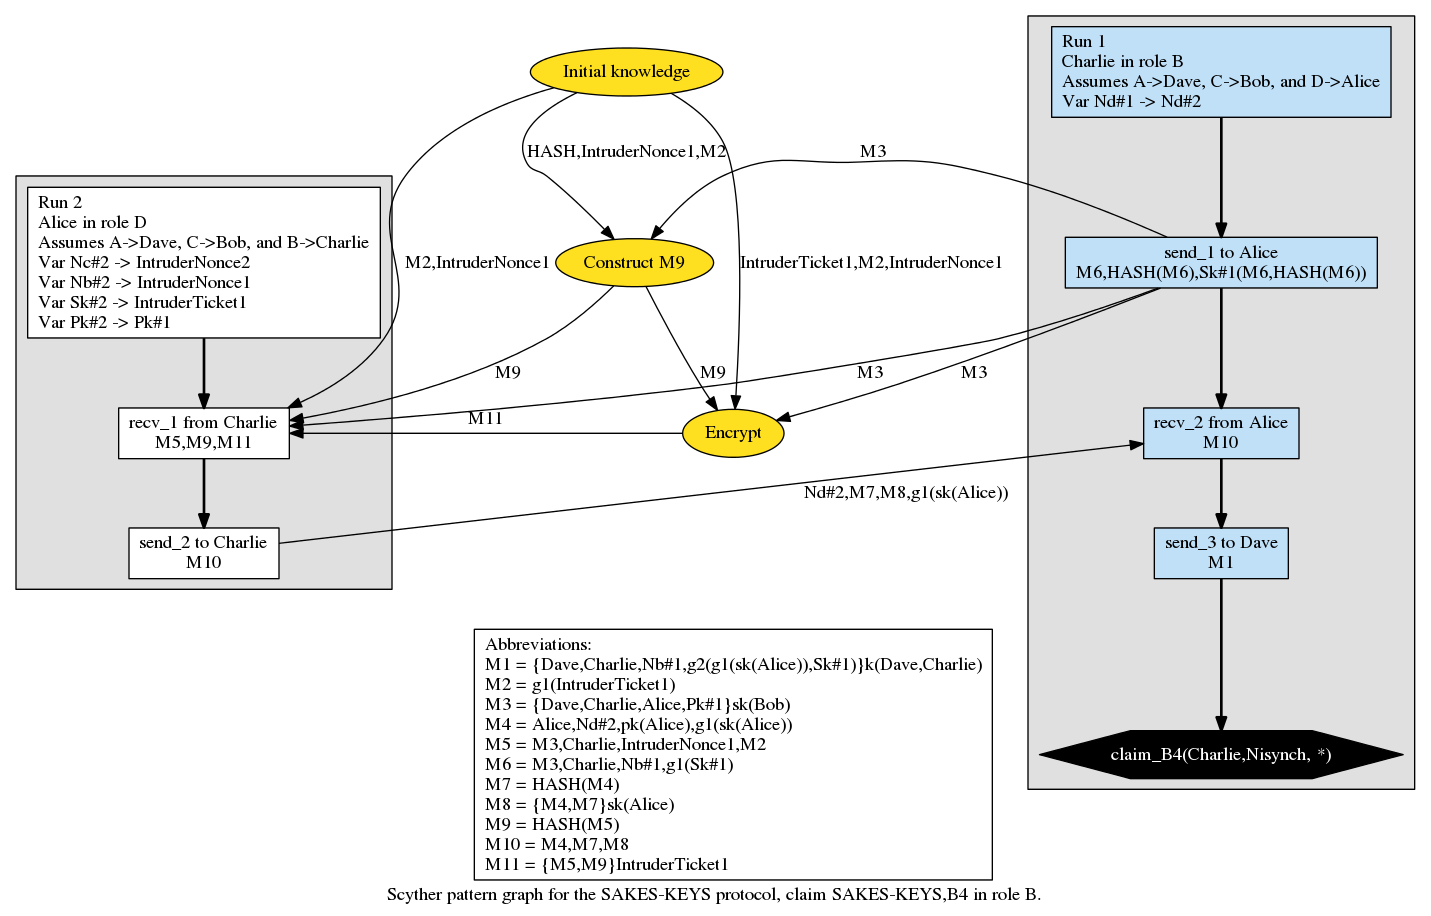
\includegraphics[scale=0.24, angle=90]{analysis/sakes-keys-b-nisynch-attack.png}
	\caption{Graph of the attack discovered on the nisynch property of the role A, B, and D from B's point of view in the key establishment phase of SAKES.}
	\label{fig:sakes-attack-keys-nisynch}
\end{figure}

\begin{figure}[h]
	\centering
	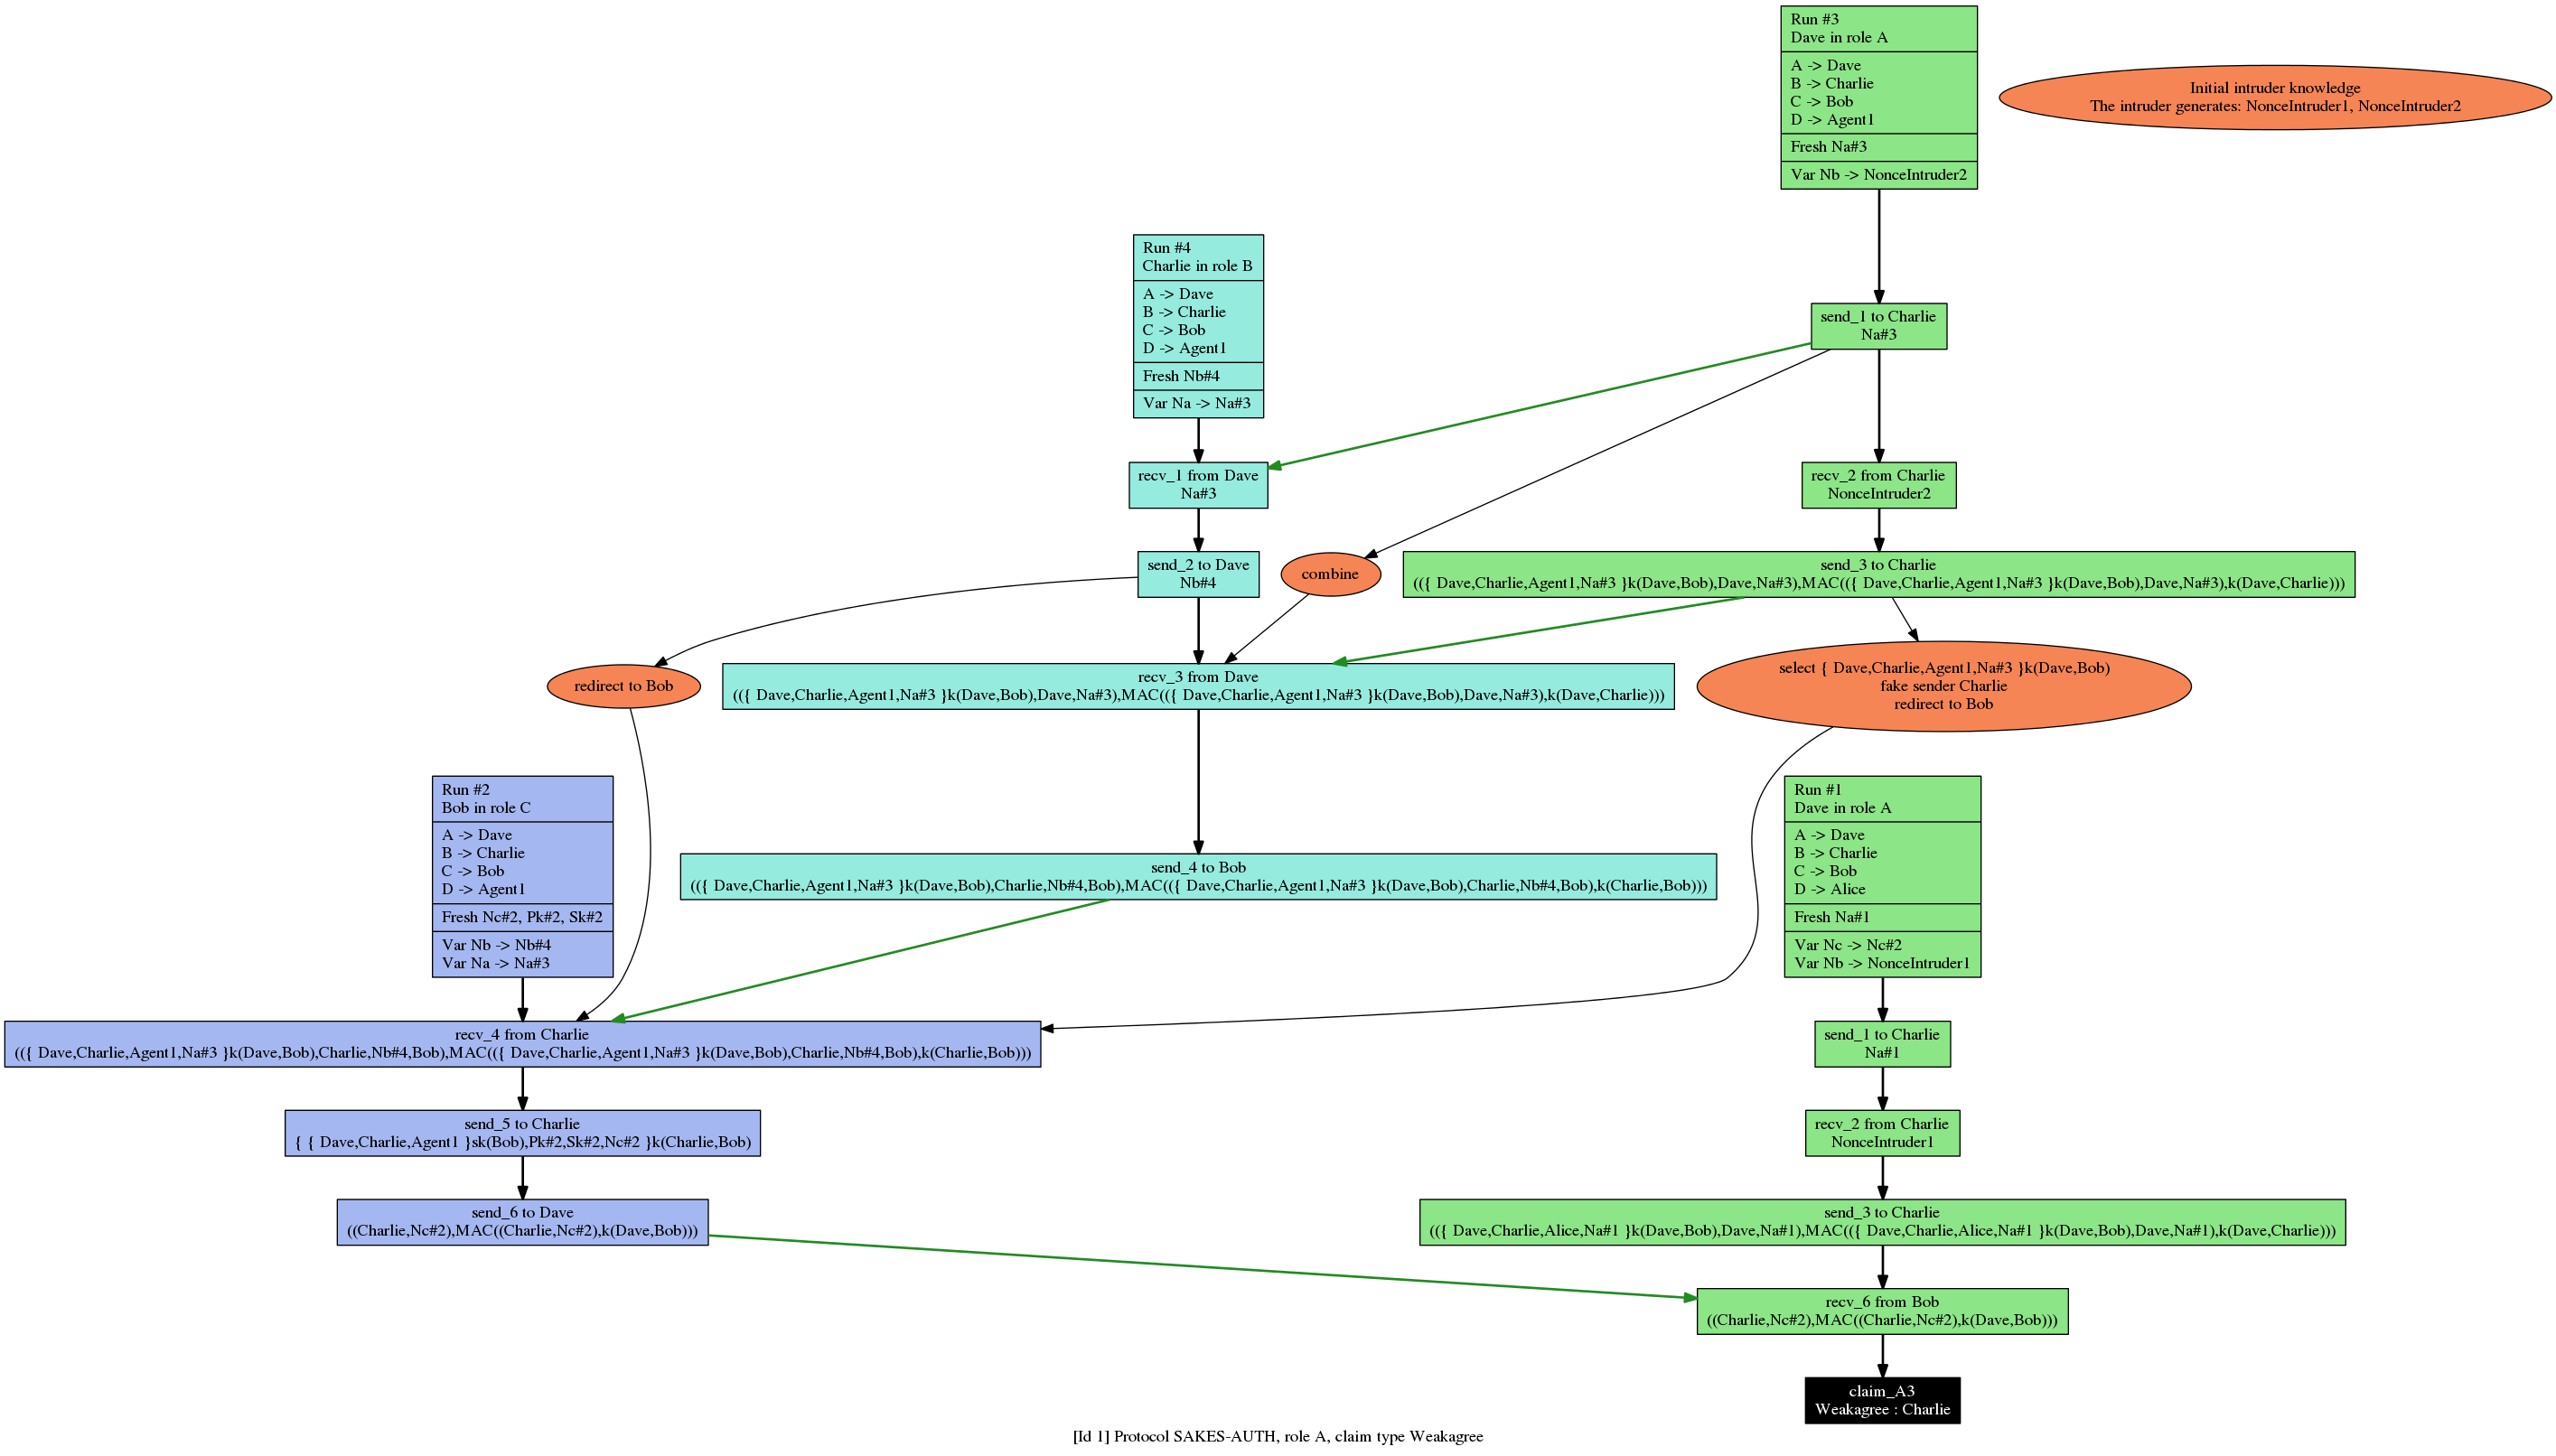
\includegraphics[scale=0.20, angle=90]{analysis/sakes-auth-a-weakagree-attack.png}
	\caption{Graph of the attack discovered on the weakagree property of the role A in the authentication phase of SAKES.}
	\label{fig:sakes-attack-weakagree}
\end{figure}

\begin{figure}[h]
	\centering
	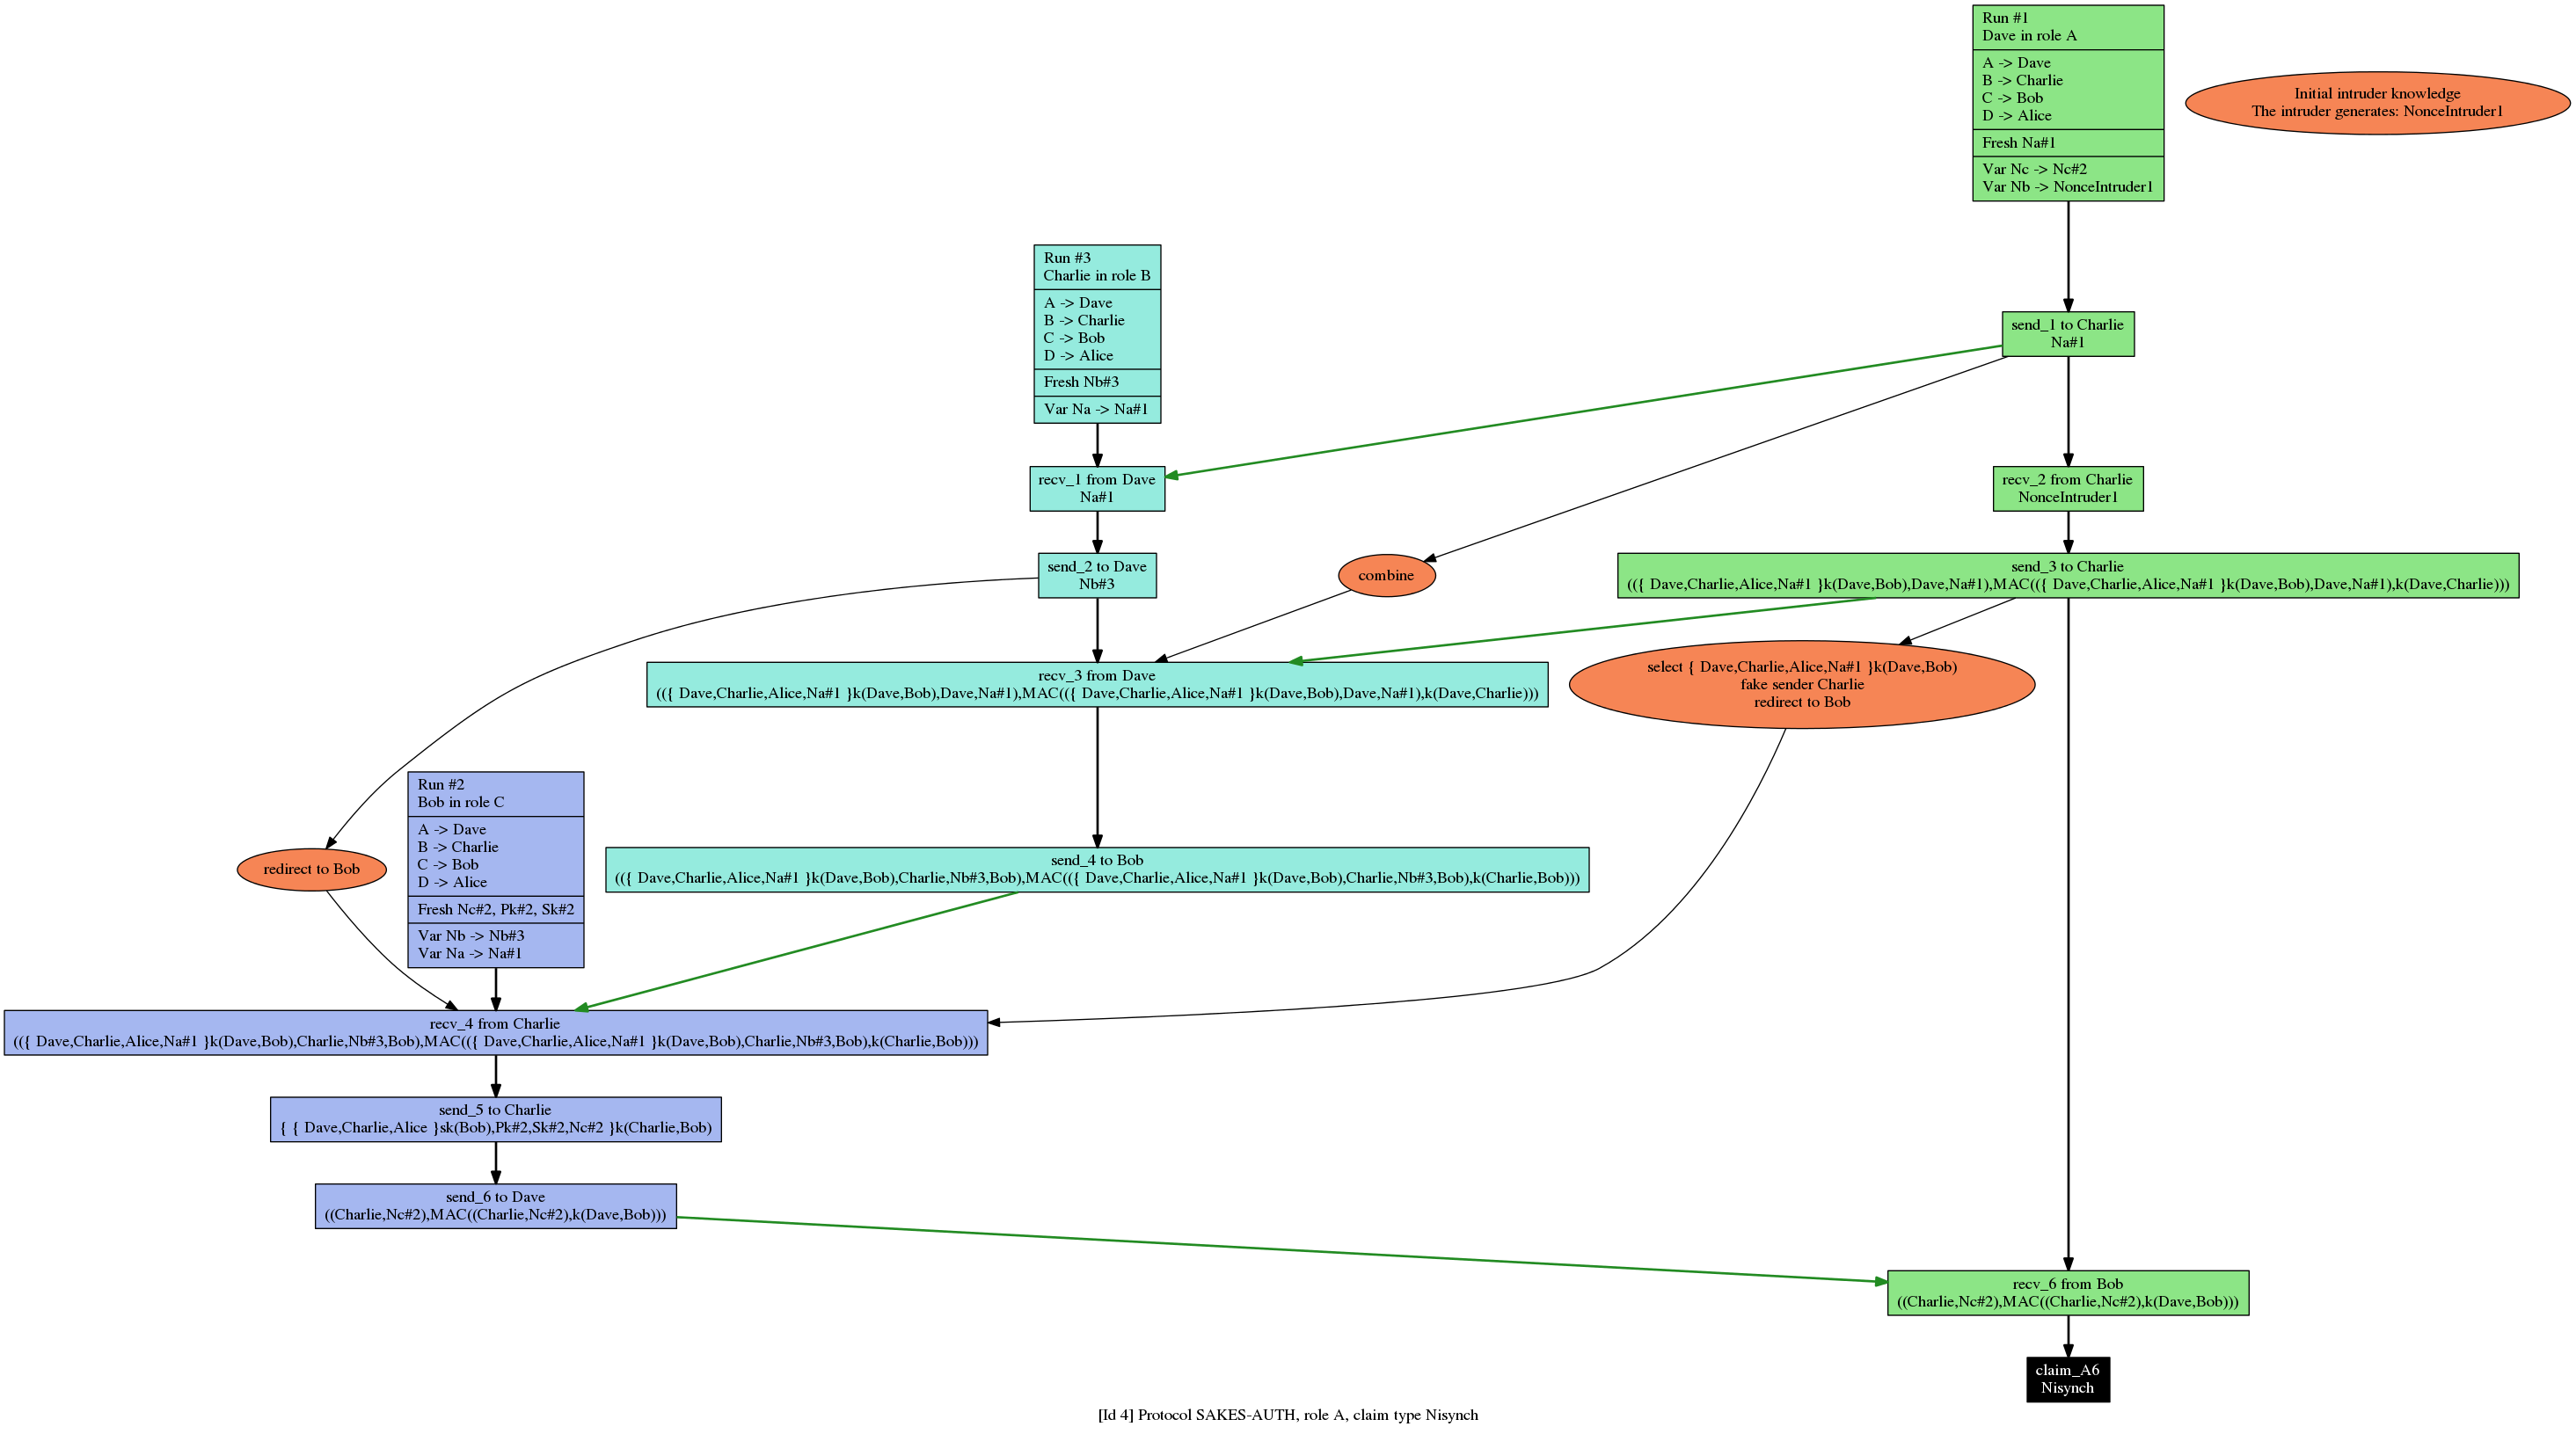
\includegraphics[scale=0.20, angle=90]{analysis/sakes-auth-a-nisynch-attack.png}
	\caption{Graph of the attack discovered on the nisynch property of the roles A, B, and C from A's point of view in the authentication phase of SAKES.}
	\label{fig:sakes-attack-nisynch}
\end{figure}

\chapter{Notations}

\section{Notations}
\label{app:notations}

\begin{tcolorbox}[title=Notations used in protocol specifications]
\begin{tabular}{ll}
\multicolumn{1}{p{1.3cm}}{\textbf{Symbol}} & \multicolumn{1}{p{4cm}}{\textbf{Meaning}}\\
A, B, C, D & Nodes\ A, B, C, D\\
$\langle{\ ...\ }\rangle{}$ & Unauthenticated message\\
$\langle{\ ...\ }\rangle{k}$ & Authenticated message with key $k$\\
$\{\ ...\ \}_k$ & Message encrypted with key $k$\\
$A \rightarrow B$ & Message sent from A to B\\
$A \rightarrow *$ & Message broadcasted from A\\
$(Pk_{node}, Sk_{node})$ & Public key pair for a node \\
$ID_{node}$ & Identity of a node\\
$AES(k, m)$ & AES encryption of message $m$ with key $k$\\
$N_{node}$ & Cryptographic nonce generated by a node\\
$X\ ||\ Y$ & Concatenation of two terms X and Y\\ 
\end{tabular}
\end{tcolorbox}





\end{document} 
